%!TEX program = xelatex
\documentclass [PhD] {uclathes}
\usepackage[toc,page]{appendix}
\usepackage[noprefix]{nomencl}
\usepackage{lscape}
\makeglossary \makeindex
\usepackage[table]{xcolor}
\usepackage{amsmath}
\usepackage{amsbsy}
\usepackage{color}
%\usepackage{cite}
\usepackage[superscript,biblabel]{cite}
\usepackage{amssymb}
\usepackage{longtable}
\usepackage{verbatim}
\usepackage{mysects}
\usepackage{chngpage}
 \ifx\pdfoutput\undefined
   \usepackage[dvips]{graphicx}
   \else
   \usepackage[pdftex]{graphicx}
   \pdfcompresslevel=9
   \fi
\usepackage{epstopdf}
\usepackage{array}
\usepackage{multirow}
\usepackage{float}
\usepackage[colorlinks,citecolor=red,linkcolor=blue]{hyperref}


\usepackage{xltxtra} % Extra customizations for XeLaTeX
\usepackage{amsmath}
\usepackage{tabularx, multirow, booktabs}
\newcommand{\otoprule}{\midrule[\heavyrulewidth]}
\usepackage{caption}
\usepackage{subcaption}
\usepackage{siunitx}


\setcounter{secnumdepth}{5}
\setcounter{tocdepth}{4}
%\linespread{1.6}%double line (1.6%) spacing, for one & half use {1.3}


%vanlew-environments

% time derivative
\newcommand{\dt}[1]{
\frac{\mathrm{d}{#1}}{\mathrm{d}t}}
\newcommand{\ddt}[1]{
\frac{\mathrm{d}^2{#1}}{\mathrm{d}t^2}}

% partial derivative (with optional numerator and required denominator)
\newcommand{\pder}[2][]{\frac{\partial#1}{\partial#2}}

% custom vector notation
\renewcommand{\vec}[1]{\mathbf{#1}}



\newcommand{\lit}{Li$_2$TiO$_3$~}
\newcommand{\lis}{Li$_4$SiO$_4$~}
\sisetup{locale = US}


% Dimensionless numbers
\newcommand{\Nu}{\mathrm{Nu}}
\renewcommand{\Re}{\mathrm{Re}}
\renewcommand{\Pr}{\mathrm{Pr}}
\newcommand{\Ra}{\mathrm{Ra}}
\newcommand{\Bi}{\mathrm{Bi}}
\newcommand{\Fo}{\mathrm{Fo}}








                        % personal LaTeX macros

%%%%%%%%%%%%%%%%%%%%%%%%%%%%%%%%%%%%%%%%%%%%%%%%%%%%%%%%%%%%%%%%%%%%%%
%
% Usually things live in separate flies.
%
% \input {prelim}                           % preliminary page info

%%%%%%%%%%%%%%%%%%%%%%%%%%%%%%%%%%%%%%%%%%%%%%%%%%%%%%%%%%%%%%%%%%%%%%%%
%                                                                      %
%                          PRELIMINARY PAGES                           %
%                                                                      %
%%%%%%%%%%%%%%%%%%%%%%%%%%%%%%%%%%%%%%%%%%%%%%%%%%%%%%%%%%%%%%%%%%%%%%%%

\title          {Shitty Dissertation Title}
\author         {Jon Thomas Van Lew}
\department     {Mechanical Engineering}
\degreeyear     {2015}

%%%%%%%%%%%%%%%%%%%%%%%%%%%%%%%%%%%%%%%%%%%%%%%%%%%%%%%%%%%%%%%%%%%%%%%%

\chair{Mohamed Abdou}
\member{member 1}
\member{member 2}
\member{member 3}



%%%%%%%%%%%%%%%%%%%%%%%%%%%%%%%%%%%%%%%%%%%%%%%%%%%%%%%%%%%%%%%%%%%%%%%%

%\dedication     {\textsl{To My loved ones \ldots without \\
%                whom I could not find the will\\
%      and courage to do this}}

%%%%%%%%%%%%%%%%%%%%%%%%%%%%%%%%%%%%%%%%%%%%%%%%%%%%%%%%%%%%%%%%%%%%%%%%

\acknowledgments {I did it all on my own}

%%%%%%%%%%%%%%%%%%%%%%%%%%%%%%%%%%%%%%%%%%%%%%%%%%%%%%%%%%%%%%%%%%%%%%%%

\vitaitem {2005} {B.S., Mechanical Engineering, Cum Laude\\ University of Arizona\\ Tucson, AZ}

\vitaitem {2010} {M.S., Mechanical Engineering \\ University of Arizona \\ Tucson, AZ}


%%%%%%%%%%%%%%%%%%%%%%%%%%%%%%%%%%%%%%%%%%%%%%%%%%%%%%%%%%%%%%%%%%%%%%%%

\abstract{It's all crap}






%%%%%%%%%%%%%%%%%%%%%%%%%%%%%%%%%%%%%%%%%%%%%%%%%%%%%%%%%%%%%%%%%%%%%%%%
\begin{document}
%%%%%%%%%%%%%%%%%%%%%%%%%%%%%%%%%%%%%%%%%%%%%%%%%%%%%%%%%%%%%%%%%%%%%%%%%
%\makeintropages



%\mymaketitlepages              % Thesis Title Page
%\mymakecopyrightpage           % Copyright Page
%\pagenumbering{roman}
%\setcounter{page}{1}
%\mymakeabstractpage            % Abstract Page
%\mymakesignaturepage           % Committee Member Signature Page
%\setcounter{page}{4}
%\tableofcontents               % Table of Contents
%\listoffigures                 % List of Figures
%\listoftables                  % List of Tables
%\chapter*{Nomenclature}

\begin{tabbing}
aaaaaaaaa\= aaaaaaaaa\kill
$A$ \>        sample cross-sectional area, m$^2$\\
$A_s$ \>        sample surface area, m$^2$\\
$b$ \>        sample thickness, m \\
$Bi$ \>       Biot number (=$hb/k$) \\
$c_p$ \>      specific heat, J/kg$\cdot$K\\
$C$ \>        capacitance, F \\
$D$ \>        electric displacement, C/m$^2$\\
$d_{33}$ \>   piezoelectric coefficient, C/N\\
$\Delta h$ \>  specific phase change enthalpy, J/kg\\
$E$ \>        electric field, V/m\\
$E_{br}$ \>    electrical breakdown field, V/m\\
$E_{c}$ \>    coercive electric field, V/m\\
$f$ \>        frequency, Hz\\
$g$ \>          gravity of Earth (=9.81 m/s$^2$) \\
$h$    \>     heat transfer coefficient, W/m$^{2}$$\cdot$K \\
$k$ \>        thermal conductivity, W/m$\cdot$K\\
$I_p$ \>      electric current, A\\
M$_A$ \>       monoclinic M$_A$ crystal phase \\
M$_B$ \>       monoclinic M$_B$ crystal phase \\
M$_C$ \>       monoclinic M$_C$ crystal phase \\
$mol\%$\>    molar fraction, \% \\
MPB \>         morphotropic phase boundary \\
$N_D$ \>      energy density, J/L\\
$Nu$ \>     Nusselt number \\
O \>       orthorhombic crystal phase \\
$p_c$ \>      pyroelectric coefficient, C/m$^2$$\cdot$K\\
$P$ \>        polarization density, C/m$^2$\\
$P_D$ \>      power density, W/L\\
$P_r$ \> 	  remnant polarization, C/m$^2$\\
$P_s$ \> 	  saturation polarization, C/m$^2$\\
$Q$ \> 	      charge, C \\
$Q_{in}$ \>     thermal energy input per unit volume, J/m$^3$ \\
PE \> 	  pyroelectric element \\
R \>       rhombohedral crystal phase \\
$R$ \> 	      resistance, $\Omega$ \\
$Ra$ \>         Rayleigh number \\
$S$ \>          side length, m \\
$s_{33}$ \>   elastic compliance, m$^{2}$/N \\
$t$ \>        time, s\\
T \>       tetragonal crystal phase \\
$T$ \>        temperature, $^o$C or K\\
$T_{Curie}$ \> Curie temperature, $^o$C\\
$x$ \>	      molar fraction of lead titanate, \%\\
$x_{3}$ \>	  strain in longitudinal direction [=$\int_{T_{C}}^{T} \! \alpha(T) \, \mathrm{d} T$] \\
$-\!\!\!\! V$ \>      volume, m$^3$ \\
$V$\>         voltage, V \\
$V_{1}$\>     voltage across capacitor, V \\
$V_{2}$\>     voltage across resistor, V \\
$W_{in}$ \>     mechanical energy input per unit volume, J/m$^3$ \\
\\

\textbf{Greek symbols} \\
$\alpha$ \>     linear thermal expansion coefficient, K$^{-1}$\\
$\delta$  \>    relative error between experimental data and model predictions, \% \\
$\varepsilon_{o}$  \> vacuum permittivity (= 8.854x10$^{-12}$ F/m) \\
$\varepsilon_{r}$ \>  relative permittivity  \\
$\eta$ \>          material efficiency, \% \\
$\nu$ \>        kinematic viscosity, m$^2$/s \\
$\rho$     \>     density, kg/m$^3$ \\
$\sigma$   \>     elastic stress, Pa \\
$\tau$$_{t}$     \>   thermal characteristic time constant, s\\
$\tau_{ij}$ \>   duration of process $i$-$j$, s\\
\\

\textbf{Subscripts} \\
$avg$ \>  refers to average \\
$b$ \>      refers to bias \\
$cold$ \>  refers to cold \\
$eff$ \>   refers to effective \\
$f$ \>      refers to fluid \\
$H$ \>    refers to high \\
$hot$ \>   refers to hot \\
$L$ \>    refers to low \\
$max$  \>   refers to maximum \\
$PE$ \>    refers to pyroelectric element \\
\end{tabbing}





%\printglossary                 % Nomenclature Page
%\mymakeacknowledgmentspage     % Acknowledgments Page
%\mymakevitapages               % Vita Page
%\mytitlefinish                 % Start a New Page for Chapter 1.

%%%%%%%%%%%%%%%%%%%%%%%%%%%%%%%%%%%%%%%%%%%%%%%%%%%%%%%%%%%%%%%%%%%%%%%%%%%
%\pagenumbering{arabic}
%\setcounter{page}{1}


% Reference sections
%%%%%%%%%%%%%%%%%%%%%%%%%%%%%%%%%%%%%%%%%%%
\chapter{Introduction} \label{sec:introduction}
%%%%%%%%%%%%%%%%%%%%%%%%%%%%%%%%%%%%%%%%%%
The controlled, sustained thermonuclear fusion of light elements is the ultimate energy source; it is inexhaustible (on our planetary scales), produces none of the greenhouse gases that are altering the climate, and avoids many of the dangers of nuclear fission. Overcoming the engineering obstacles to tame the fusion reaction is the greatest technological challenge of our generation. A recently-published book by Dr. Francis Chen provides an excellent coverage of the basics of fusion energy, the reactions, our present understanding of the fusion plasma, and the role fusion energy can play in the global energy market.\cite{Chen2011} 

In this dissertation, I will begin by presenting only an extremely brief summary of the main points on the background of general fusion technology as necessary for establishing a common language that will be used in the rest of the document. Slightly more background will be given for the fusion nuclear technology that are immediately relevant to the research I have performed, specifically the breeder blanket of a fusion reactor.

\section{The Basics of Nuclear Fusion and Tritium Breeding}\label{sec:fusion-basics}

The fusion reaction assumed to be the first choice demonstrable fusion power plants involves the two hydrogen isotopes of deuterium and tritium. The deuterium-tritium (DT) reaction has a high reaction probability at the lowest ion temperature and a high energy yield. Alternative fusion reactions of two deuterium atoms or a deuterium atom with helium-3 are advantageous in other regards, such as no radioactive byproducts or fuel availability, but their relatively-higher ion temperature preclude them from current consideration.\cite{abdou} The DT reaction proceeds as
\begin{align}
	\mathrm{D} + \mathrm{T}&\xrightarrow{}\ ^4\mathrm{He}+\mathrm{n}+17.58\ \text{MeV} \label{eq:dt-reaction}
\end{align}

Of the two isotopes fused, deuterium ($D$, or $^2$H) is a stable isotope and is naturally occurring in an average abundance of 0.015 mole percent in water on Earth. To demonstrate just how plentiful deuterium is as a fuel source, there is approximately 100 million billion kilograms of deuterium in the Earth's oceans. If all energy on Earth were produced from DT fusion power plants, there would be enough deuterium to outlast the lifetime of our sun. It is safe to say we will not exhaust our deuterium sources on Earth.

Tritium ($T$, or $^3$H), however, is radioactive with a half-life of only about 12.32 years; any naturally occurring tritium decays at such a rapid pace it will never accumulate to an appreciable amount on Earth. If tritium is to be used as a fuel in a fusion power plant, it must be generated artificially -- thus the need for the so-called tritium breeding blankets in fusion reactors. In-situ generation of tritium in a fusion reactor is possible with the assistance of lithium. Natural lithium will interact with neutrons as
\begin{subequations}\label{eq:lithium-t}
\begin{align}
	\mathrm{n} + \ ^7\mathrm{Li} &\xrightarrow \ \mathrm{n}+\alpha + \mathrm{T} -2.47\ \text{MeV}\label{eq:li7-t}\\
	\mathrm{n} + \ ^6\mathrm{Li} &\xrightarrow \  \alpha + \mathrm{T} +4.78\ \text{MeV} \label{eq:li6-t}
\end{align}
\end{subequations}
where we have used the common short-hand of $\alpha$ in place of the helium nucleus. The cross-sections of the lithium reactions are given in Fig.~\ref{fig:li-xsects}. Note the exothermic lithium-6 reaction (a neutron of any energy will incite the transmutation) and the threshold energy required of the incident neutron in the endothermic lithium-7 reaction. The exothermic reaction is also the source of energy that will ultimately generate the electricity of the fusion power plant.

\begin{figure}[ht]
	\centering
	\includegraphics[width=0.6\textwidth]{chapters/figures/breeding_xsecs} 
	\caption{Cross-sections of various blanket materials. Note the threshold for the $^7$Li and neutron multiplying reactions.}
	\label{fig:li-xsects}
\end{figure}

Lithium, like deuterium, is quite abundant on Earth. To make the point clear, there is enough lithium accessible in the Earth's crust to generate tritium for 30 million years worth of DT reactions if they were providing all of humanity's electricity.\cite{Chen2011}. Thus lithium is an excellent candidate for generating the tritium necessary to self-sustain the fusion reaction in a power plant. Lithium is the main material component of tritium breeder blankets -- the form of lithium as it exists in the breeding blanket is a source of continued research.

At present there are two main avenues of tritium breeder designs: those containing liquid or solid lithium. Many of the functional requirements are similar between the two designs but their implementation is quite different. While much research has been -- and continues to be -- performed on the liquid breeder design (for examples, see Refs.~[cite many liquid breeder papers]), the work of this dissertation focuses solely on a particular solid breeder design. In the next section I will refer to the breeding blanket almost exclusively as the ``solid breeder'' though it should be understood that many of the generic features and requirements of the solid breeder are shared with its sister design, the liquid breeder.

\subsection{Breeding Blanket for Fusion Reactors}


\begin{figure}[ht]
	\centering
	\includegraphics[width=1\textwidth]{chapters/figures/demo} 
	\caption{An example design of a DEMO reactor with solid breeder blankets shown as inboard (IB) and outboard (OB) blanket components.}
	\label{fig:demo}
\end{figure}

\begin{figure}[ht]
	\centering
	\includegraphics[width=0.85\textwidth]{chapters/figures/solid_breeder_sketch} 
	\caption{Sketch of a typical unit of a pebble bed tritium breeding zone. The pebble bed is cooled with contact to the containing structure.}
	\label{fig:solid-breeder-sketch}
\end{figure}

The breeder blanket is a pivotal piece of engineering technology upon which the success of a fusion power plant rests. The successful operation of a breeder will see the device capture the neutrons ejected from the fusion reaction to generate fuel for future reactions, breed and recover fuel for the fusion reaction, act as shield to other sensitive equipment, and convert energy into extractable heat for electricity production. Figure~\ref{fig:demo} shows an example sketch of a demonstration (DEMO) fusion reactor and the relative location of the breeder blanket modules as they face the plasma in the torus of the tokamak. 

From the inception of the solid breeder concept in 1975 by Abdou\etal\cite{Abdou1975c}, designs have evolved significantly to meet the requirements of operation in the harsh fusion environment. Currently, the reference solid breeder design incorporates packed beds of ceramic pebbles (spherical particles) that are filled into containment structures of sizes optimized for thermophysical and tritium responses. The main features of many reference designs is illustrated in the sketch of Fig.~\ref{fig:solid-breeder-sketch}.

The pebble bed of Fig.~\ref{fig:solid-breeder-sketch} is contained by a low-activation steel which serves as both mechanical and thermal boundaries for the ensemble. The breeding blanket will experience high volumetric heating (resulting from secondary $\gamma$ rays and the kinetic energy of neutrons that are carrying away approximately 80\% of the fusion reaction) and temperatures will be allowed to increase to approximately 900~\celsius. The heat is conducted via the purge gas and inter-particle contacts between pebbles to the structural material. A high pressure (approximately 8 MPa) helium coolant is then run through the structure. The coolant will heat to approximately 500~\celsius before exiting the blanket, maintaining the structure below structural temperature limits. The heat carried away by the coolant ultimately works its way into an electricity-producing cycle. 

As the neutrons bombard the lithiated ceramic, tritium is produced internal to the pebbles. The tritium atoms work their way slowly to the surface of the pebble whereupon they desorb into a passing, low-pressure (approximately atmospheric) helium purge gas. Tritium that transmutes from the lithium inside the pebble will diffuse slowly through the bulk until reaching a grain boundary. Tritium moves relatively quickly along the grain boundary until reaching a surface of open porosity where it may desorb into the passing purge gas.\cite{Federici1990} The low-speed purge gas is pumped through the pebble bed to extract the tritium generated and transport it out of the blanket for processing. 

The dual role of the breeding blanket to generate heat and tritium forces a specific operational temperature window for the ceramic pebble beds. The low end of the temperature window is governed by a minimum temperature for acceptable release rates of tritium from the ceramic to the purge gas; the value is generally set around 300~\celsius. The upper limit of the temperature window is chosen to avoid sintering of the lithiated ceramic, giving the approximately 900~\celsius limit. Based on current understanding of tritium release from the pebble, as grains grow during sintering of the ceramics the tritium release rate is expected to decrease.

\begin{figure}
        \centering
        \begin{subfigure}[b]{\doubleimagewidth}
                \includegraphics[width=\textwidth]{chapters/figures/keff-pressure}
                \caption{Effective conductivity of ceramic pebble beds is dependent on the pressure of the interstitial gas, a minimum of about $k_\text{eff} = 1$~W/m-K in vacuum.}
                \label{fig:keff-pressure}
        \end{subfigure}%
        
          %add desired spacing between images, e. g. ~, \quad, \qquad, \hfill etc.
          %(or a blank line to force the subfigure onto a new line)
        \begin{subfigure}[b]{\doubleimagewidth 	}
                \includegraphics[width=\textwidth]{chapters/figures/lit-keff-exp}
                \caption{The effective conductivity of pebble beds is weakly dependent on external mechanical pressure and is always approximately $k_\text{eff} = 1$~W/m-K in helium.}
                \label{fig:keff-lit}
        \end{subfigure}
        \caption{Effective conductivity of lithium ceramics.}\label{fig:keff}
\end{figure}

The size of breeder region is limited by the operational temperature window that must be held in spite of the the poor effective conductivity of packed beds of ceramic pebbles. The conductivity is experimentally shown to be a weak function of external pressure but can generally no greater than about \si{1 W/{mK}} -- for well-packed beds. Because the effective conductivity and packed bed-wall interface conductance is predominately a contact conduction, disruptions to the packing structure will have considerable impact on the heat transfer of the packed bed.

Moreover, as nuclear energy is deposited into the poorly-conductive ceramic breeder material and the temperature climbs well above the containing structure, it will confine the thermal expansion of the lithium ceramic and lead to mechanical stresses at the points of contact of the individual pebbles in the packed bed. Engineering design issues surrounding this thermally-induced stress is of great concern to researchers and will be the focus of much of this report.





 % the fusion reaction deposits   The nuclear heat generated in the pebble bed solid breeder will heat the ceramic pebbles to maximum temperatures of approximately 900~\celsius. The heat of the pebbles is transported through them via conduction through inter-particle contacts, conduction through the purge gas into neighboring particles, and ultimately through contact with the containing structure. The box structure surrounding the solid breeder will have high pressure (\si{8~MPa} in many current designs) 


























\section{Motivation}\label{sec:motivation}
\subsection{Pebble Bed Integrity, Thermophysics, and the Role of Modeling}\label{sec:intro-bed-integrity}
and continue operating despite the environment without being replaced or actively maintained. Its important that the solid breeder not simply survive the thermal and mechanical demands of the reactor environment but continue to release predictable and acceptable amounts of tritium. Increasingly reliable and accurate models are crucial in the design of operational solid breeder blanket technologies. In this dissertation, we advance the field of solid breeder modeling with the introduction of new techniques and tools.



The pebble bed will experience a constrained thermal expansion as the hot ceramic pebbles press against the relatively cooler container. The restricted thermal expansion of the pebble bed causes an external pressure on the pebble bed. The external pressure may lead to a number of phenomena that disrupt the initial packing -- and by extension the initial predictions of thermal and mechanical properties -- of the pebble bed. For one, in experiments of even well-packed ensembles of pebbles, the beds show an apparent plastic strain of rearranged packing that increases with maximum historical stress on the bed.[cite Chunbo and Reimanns experimental papers] Without careful engineering and packing of the virgin pebble beds, plastic strain in the pebble bed will directly lead to the formation of gaps between the pebble bed and containing structure. Depending on the configuration of the solid breeder design, the gap could cause a tremendous loss of heat transport from the pebble bed to the coolant. Furthermore, any gaps formed in the blanket could lead to more neutron leakage and decreased tritium breeding ratios and detriment to the blanket's shielding function.

Additionally, assuming that the plastic strain is removed from the pebble bed, the thermally-induced pressure on the pebble bed will be balanced by the individual pebbles pressing into each other at small points of contact. The small area over which the contact forces are applied leads to stresses which may crush individual pebbles in the ensemble. With the potential accumulation of many cracked/crushed individual pebbles, the overall packing structure is again altered. Depending on the extent of crushing, the response of the pebble bed may be as benevolent as a negligible decrease in effective thermal conductivity or malevolent as a loss of physical contact and heat transport from the pebble bed to the coolant. 

Finally there are long-term effects expected in the materials experiencing prolonged exposure to cycling irradiation, heat, and stress. Thermal ratcheting, swelling, sintering, or thermally-induced creep can lead to evolutions in thermophysical properties even in the absence of cracked pebbles. As the thermophysical properties evolve, global or local bed temperatures change and ultimately the tritium release characteristics of the bed deviate from any prediction one may have had from the initial packing of the ceramic pebble bed. 

In our group we are most focused on maintaining tritium breeding characteristics of the pebble bed at desirable levels and thus maintaining temperatures in the breeding region. Alleviating any of the issues that may plague the ceramic breeder all boil down to requiring temperature control via an understanding and of the morphological changes of the ceramic packed beds and their interaction with the interstitial purge gas and structural container. [say how temperature control is possible with better models]In this work we introduce enhancements and new elements to build upon the understanding from ceramic breeder models of past research efforts. 







% Control of the manufacturing processes of the ceramic pebbles permits manufactureres to custom vary characteristics, such as the pebble's:
% \begin{itemize}
% \item tritium retention and release properties.
% \item Lithium density
% \item Opened- and closed-porosity
% \item Nominal diameter
% \item and, indirectly, crush strength. 
% \end{itemize}
% However the characteristics of the pebble are often coupled. For instance, for the sake of tritium management the open porosity of the pebble is often increased. But this comes at the expense of a decreased crush strength of the pebble. Because of the relatively weak crush strength distributions among batches of pebbles as well as the value of stresses predicted in the pebble bed, it is inevitable that during operation in the fusion environment individual pebbles will `fail' in the ensemble. Designers of lithium ceramic tritium breeding blankets must mitigate pebble failure but also anticipate the breadth and magnitude of effects that some unavoidable failure will have on macroscopic properties.



% [EDIT: THIS PARAGRAPH IS NOT NECESSARY? I DON'T NEED TO MAKE THE CASE FOR USING DEM. I JUST NEED TO EXPLAIN THE MODEL]The volume of a pebble in a tritium breeder is on the scale of 10$^{-9}$~m$^3$ while the typical container volume can be on the order of 10$^{-2}$~m$^3$\cite{Cho2008}.  Thus a single breeder volume will house upwards of $N = 10^7$ pebbles. Statistically then, the behavior of any single pebble seems insignificant and instead the entire ensemble of pebbles may be treated as a continuous media. Continuum theory for the is the basis of finite element method models that have been able to predict thermo-mechanical behavior with reasonable accuracy\cite{DiMaio20081287,Zaccari20081282,Gan:2009vn}. However, after the pebble beds are placed into the fusion environment they will be required to operate for long duty times without maintenance. Thus, as time progresses the accumulation of individual failed pebbles will eventually have consequences for the macroscopic thermo-mechanics.  and no continuum theory exists to account for this. Instead, we turn to the discrete element method to provide a solutino.









\subsection{Scope of the Work}\label{sec:intro-scope-of-work}
The objective of this dissertation is to develop numerical models of ceramic pebble beds, based on first principles and experimental observations, to simulate the hysteritic evolution of pebble bed morphology and predict the subsequent changes to heat transport characteristics after thermally-induced damage to pebbles. The numerical tools are constructed in the following progression: 1. Transient DEM code of inter-particle interactions is employed to simulate packed bed restructuring in the wake of crushed pebbles in the ensemble -- and the effective thermal conductivity following the restructuring, 2. Transient, volume-averaged equations of Navier-Stokes and energy of the helium purge gas are coupled to the DEM model of pebbles to simulate conjugate heat transfer and the interstitial fluid influence on thermophysical properties after crushing events, 3) Complete simulations of the tortuous path of helium purge gas with lattice-Boltzmann models (based on the packing structure determined in DEM simulations) to expose flattened temperature profiles due to laminar mixing in the pebble bed. 

A thorough understanding of the evolution of pebble bed morphology and the impact on thermophysical properties is critical for solid breeder designers. The understanding allows for temperature control of breeder pebble beds over the entire lifetime of the blanket which is crucial to the function of the solid breeder for tritium and energy generation. Thus we aim to provide designers of packed beds with tools to understand how packing states may evolve from time-dependent phenomena (e.g. sintering, creep, pebble cracking, etc.). These phenomena may, for instance: decrease the effective thermal conductivity which will raise bed temperatures beyond initial predictions, produce isolated pebbles which will sinter and potentially decrease tritium release rates, or even form gaps between pebble beds and containing structures leading to divergence from properties of the initial packing of the bed.

The objective of this work fits into the broader mission of our research group in the UCLA Fusion Science and Technology Center to develop and apply complete numerical models of ceramic pebble bed solid breeder modules. Any complete numerical model for a pebble bed would require the interaction of many sub-models or sub-functions operating at disparate scales. To demonstrate, a possible top-level algorithm could proceed in the following way: To begin, one must have knowledge of the interaction of the pebble bed with the containing structure as they exist in a fusion environment. The interactions are generally analyzed via the finite element method to find internal stresses and temperature fields of the entirety of the pebble bed and surrounding container. After the internal fields are mapped into the bed, one would use the discrete element method (DEM) to interpret the macroscopic stress fields into the inter-particle forces. With the inter-particle forces and total absorbed thermal energy calculated, a prediction of the initiation and evolution of morphological changes (i.e. crushed pebbles, sintering, creep, etc.) to each computational volume. Following this, DEM would calculate new effective properties as a result of the morphological changes to the pebble bed region. Finally, the updated bed properties would feed back into the FEM formulation to update calculations in the macroscopic stress fields. While a suite of integrated numerical tools that follows this example algorithm is the ultimate goal of our group, the work of this dissertation is focused entirely on the development of pebble-scale simulations that are predominately in the realm of the discrete element method.

In the following subs-sections, we briefly outline the studies fitting into the scope of this dissertation. 

\subsection*{Discrete Element Method Study on the Evolution of thermo-mechanics of a Pebble Bed Experiencing Pebble Damage}
In the first study of \cref{sec:dem-studies}, we analyze the effective thermal conductivity of a pebble bed assuming different fractions of pebbles in the ensemble are completely crushed. The focus of this study is to 1) determine the extent of change, in aggregate, to ensemble properties due to individual pebble crushing, 2) relate the changes in effective conductivity to quantifiable pebble-scale properties (e.g. contact force, coordination number, etc.), 3) use the results to create guidelines for designers to anticipate acceptable limits of pebble loss from a thermal management point of view. For the DEM tools used in this study, the only mode of heat transfer considered is conduction between the solid particles. 


\subsection*{Coupling DEM Models of Ceramic Breeder Pebble Beds to Thermofluid Models of Helium Purge Gas Using Volume-averaged CFD}
In a fusion breeder, the helium purge gas winding through the interstitial gaps of the pebbles has a substantial contribution to overall heat transfer.\cite{Reimann:2002mi,Abou-Sena2005} The model of \cref{sec:dem-studies} is improved to include the flowing interstitial gas. In \cref{sec:cfd-dem-studies}, we continue to employ our DEM tools to provide particle-scale information such as contact force, but couple the pebbles to a volume-averaged computational fluid dynamics (CFD) code for the conjugate heat transfer simulation. The coupled CFD-DEM model is used to again simulate the heat transfer in packed beds of ceramic spheres that experience pebble crushing -- but now with a focus on highlighting the impact of a flowing interstitial helium purge gas when pebbles are crushed.


\subsection*{Lattice-Boltzmann Method Integrating DEM Packing Structures to Study Laminar Mixing}
The models to account for helium purge gas employed in the studies of \cref{sec:cfd-dem-studies,sec:applied-studies} assume effective drag or heat transfer coefficients for pebbles in a computational volume and then include the pebble influence through effective source/sink terms in the momentum and energy equations. The volume-averaged approach allows for simpler meshing of the fluid volume while still retaining much of the physical realism of the system. Complete models of the conjugate heat transfer of both the fluid moving through the tortuous interstitial gaps pebble beds pressing each other with small contact areas are intractable with current computational hardware and finite-element modeling techniques. To overcome deficiencies in computational power, in \cref{sec:modeling-lbm}, we apply a relatively new technique wherein a lattice-Boltzmann algorithm solves for complete flow fields and conjugate heat transfer of helium winding through a packed bed. The lattice-Boltzmann method (LBM) is a non-traditional fluid simulation technique that allows us to resolve pebble/pore-scale momentum and energy transfer. The LBM approach is applied to the same pebble beds analyzed in \cref{sec:cfd-dem-studies} to provide comparison between the two modeling techniques. Furthermore the LBM model, accounting for the complex helium purge gas pathways, provides more insight to the influence of helium on the heat transfer in the heat transfer of packed beds.





\subsection*{Modeling Tools to Study Coolant Designs of ITER Solid Breeder Module Volumes}
In the study of \cref{sec:applied-studies}, we apply our coupled helium-pebble computational tools to the analysis of ITER-relevant solid breeder geometries. In this study we consider the combined effects of pebble crushing, packing restructuring due to both gravity and the unbalanced force network in the pebble bed, and convection from helium purge gas on temperature profiles in solid breeders for different breeding configurations. Heat transfer out of the pebble bed relies on maintaining good pebble-pebble and pebble-wall contact. However, physical contact is interrupted to different degrees when a pebble bed responds to various amounts of individual crushed pebbles. Furthermore, the restructuring of the pebble bed after a pebble crushing event is, in part, dependent on gravity forces acting upon each pebble in the ensemble. We investigate two representative pebble bed configurations where heat is removed from the bed via inter-particle conduction, convection of purge gas, and contact between the pebble bed and its container. In the first, the coolant containing structural walls (heat transfer walls) are oriented parallel to the gravity vector. In the second configuration, the heat transfer walls are perpendicular to the direction of gravity. To simulate a crushed pebble, we replace the pebble with many smaller, non-cohesive elements while maintaining mass-conservation between the original solid pebble and crushed fragments. The fragments are then free to resettle into interstitial gaps and the rest of the bed resettles as determined by forces from gravity, contact of neighboring particles, and even the small influence of the moving purge gas. The thermo-fluid interaction with the helium purge gas will be included with volume-averaged Navier-Stokes and energy equations. The representative solid breeder volumes will be compared with respect to their temperature peaks and profiles and how those temperatures vary as a function of the percentage of crushed pebbles in the ensemble. The results can be used to optimize solid breeder pebble bed designs through the choice of breeding zone orientation relative to the gravity vector.



\chapter{Dissertation Outline}
The path toward the modeling efforts outlined for the scope of this work is not a clear, straight line. To accomplish the goals set forth -- attempting to discuss them in the most clear and accurate way possible -- this dissertation is broken up into five major parts following their logical partitions. This section, Part I, provides the introduction and motivation behind the work. In Part II, (containing Chapters: \cref{sec:hertz-theory,sec:modeling-state,sec:survey-packed-beds}) we survey the state of the art in analysis of ceramic pebble beds, contact mechanics, and modeling thermal and mechanical interactions of particles in packed beds and fluids moving interstitially.  In Part III, (containing Chapters: \cref{sec:modeling-dem,sec:modeling-cfd-dem,sec:modeling-lbm}) we outline the numerical methodology and development of modeling tools we shall use in the study and analysis of pebble beds and their evolving morphology due to external loads. We compartmentalize the numerical tools into three parts, namely: the discrete element method (DEM), coupled computational fluid dynamics and the discrete element method (CFD-DEM), and a lattice-Boltzmann method (LBM) we integrate with DEM. The development of the tools is assisted with theoretically- and experimentally-based studies on individual pebbles in an ensemble. The newly developed enhancements to the numerical tools are studied before their inclusion in the toolkits. We work through the results of the promised studies in Part IV (\cref{sec:cfd-dem-studies,sec:dem-studies,sec:lbm-studies,sec:applied-studies}). Finally, in Part V, we discuss the next steps to be taken that we identify as critical next steps -- but beyond the scope of this dissertation -- for the modeling tools. In addition, other research avenues that have been opened by the tools introduced and their potential impact are discussed here.
%\input{chapters/background-discussion.tex}


% Content
\input{chapters/background-analysis.tex}
%\input{chapters/modeling-pressure-drop.tex}
%%%%%%%%%%%%%%%%%%%%%%%%%%%%%%%%%%%%%%%%%%
\chapter{Heat transfer in packed beds} \label{ch:modeling-heat-transfer}
%%%%%%%%%%%%%%%%%%%%%%%%%%%%%%%%%%%%%%%%%%
This section covers a discussion of different modes of heat transfer experienced by a pebble in a packed bed. The main modes are conduction to neighbors and convection.




\section{Single particle modes of heat transfer}

\begin{figure}[t]
	\centering
	\caption{Each ceramic pebble in a fusion reactor will experience multiple modes of heat transfer.}
	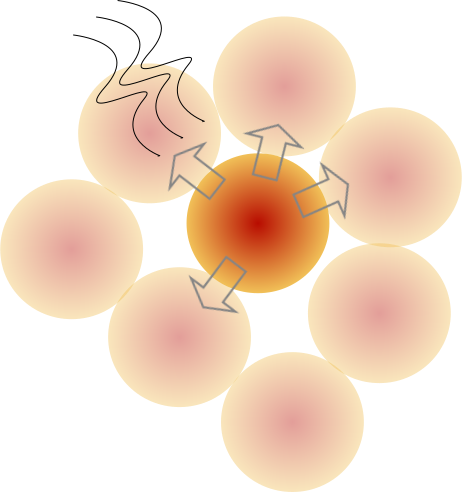
\includegraphics[width=0.75\textwidth]{chapters/figures/pebble-complete-heat-transfer}\label{fig:peb-comp-ht}
\end{figure}

The transient energy balance for an irradiated pebble, shown in Fig.~\ref{fig:peb-comp-ht}, in a packed bed with flowing interstitial gas is given by Eq.~\ref{eq:single-pebble-energy},

\begin{equation}\label{eq:single-pebble-energy}
	\rho V C \frac{\mathrm{d}T}{\mathrm{d}t} = \dot{Q}_g + \dot{Q}_\text{conduction} + \dot{Q}_\text{convection} + \dot{Q}_\text{radiation}
\end{equation}

We begin with the lumped capacitance assumption that internal temperature gradients inside of the solid particle are negligible thus we can neglect diffusion terms in the solid. The validity of that assumption for the ceramic pebbles in fusion reactors will be discussed in detail in \S\ref{sec:ht-jeffreson-correction}. The terms on the right-hand-side of Eq.~\ref{eq:single-pebble-energy} are:

\begin{enumerate}
\item Conduction through the stagnant fluid between two point- or non-contacted particles.
\item Conduction through the stagnant fluid between two area-contacted particles.
\item Conduction through the contact area between two area-contacted particles.
\item Conduction through the fluid in void space. 
\item Radiation between the surfaces of two particles.
\item Radiation between adjacent voids.
% \item Convective heat transfer between fluid and solid particles.
% \item rate of energy generated internal to the pebble,
% \item rate of conduction between neighboring pebbles in their regions of contact, 
% \item rate of convective heat transfer with the interstitial helium gas (which includes energy carried far downstream or redeposited to neighboring pebbles), and
% \item rate of radiative exchange between local solids.
\end{enumerate}

% In this section we will provide a brief overview of all the modes of heat transfer to provide an overview of the importance and impact of each mode. For cases when more detail is needed, the details will be expounded in their own complete sections.

% \subsection{Heat generation}

% Nuclear deposition of energy is handled in a straightforward manner. With a known volumetric energy generation rate, $q'''$ prescribed by, for instance, the neutron heating in the volume, the heat generation rate for this particle is simply

% \begin{equation}
% 	\dot{Q}_g = q'''V
% \end{equation}




%%%%%%%%%%%%%%%%%%%%%%%%%%%%%%%%%%%%%%%%%%
%\section{Single particle heat transfer}

\begin{figure}[t]
	\centering
	\caption{Each ceramic pebble in a fusion reactor will experience multiple modes of heat transfer.}
	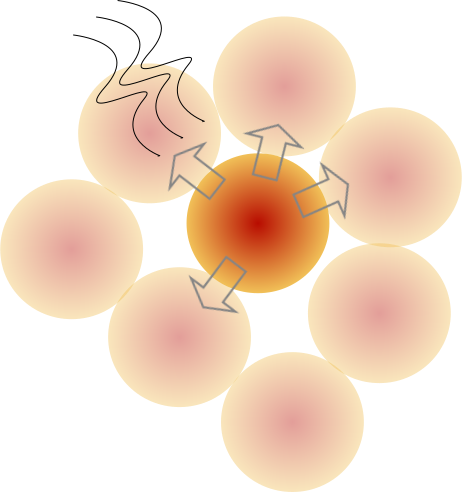
\includegraphics[width=0.75\textwidth]{chapters/figures/pebble-complete-heat-transfer}\label{fig:peb-comp-ht}
\end{figure}

Shown in Fig.~\ref{fig:peb-comp-ht} are all the modes of energy transfer on a pebble inside the fusion reactor. There is:

\begin{enumerate}
\item energy generated internal to the pebble caused by nuclear heating,
\item conduction internally of the solid material to the surface of the pebble, 
\item conduction between neighboring pebbles at their areas of contact, 
\item radiation between neighboring solids, and 
\item convective heat transfer with the interstitial helium gas (which includes energy carried far downstream or redeposited to neighboring pebbles).
\end{enumerate}









\subsection{Nuclear heating}

Nuclear deposition of energy is handled in a straightforward manner in the DEM computations with a simple source term on the energy balance equation. 












\subsection{Conduction through the solid}\label{sec:ht-pebble-conduction}

Before considering the heat equation in a sphere, it is instructive to first consider the simpler problem of a one-dimensional slab with volumetric heat generation, $q_g'''$ and convective cooling at the surfaces. The geometry is shown in Fig.~\ref{}.

Assuming we can find the Nusselt number for the convective cooling, we write the heat flux from the surface to the fluid as

\begin{equation}
	q_s'' = h(T_s - T_f)	
\end{equation}

where $T_f$ is the bulk fluid temperature and $T_s$ is the surface temperature. At steady-state the amount of heat moved across the fluid-surface interface must necessarily be equal to the total amount of heat generated into the slab. Therefore,

\begin{equation}
	q_w'' = q_g'''L = h(T_f-T_s)
\end{equation}

where $L$ is the half-width of the slab. For the sake of discussion, we re-write the above in terms of the temperature delta from surface to fluid in terms of nuclear heating,

\begin{equation}\label{eq:fluid-delta}
	T_f-T_s = \frac{q_g'''L}{h}
\end{equation}

Inside the slab, at steady-state the energy equation is simply a balance of heat conduction and nuclear generation. 

\begin{equation}\label{eq:nuclear-heating-slab-ode}
	0 = k\frac{\mathrm{d}^2T}{\mathrm{d}x^2} + q_g'''
\end{equation}

The boundary conditions are symmetry about the centerline and known surface temperature

\begin{align}
	q_{L=0} &= 0 \\
	T(L) &= T_s
\end{align}

The ODE of Eq.\ref{eq:nuclear-heating-slab-ode} is solved with simple separation and integration. When the boundary conditions are applied we have

\begin{equation}
	T(x) = \frac{q_g''' L^2}{2k}\left(1-\frac{x^2}{L^2}\right) + T_s
\end{equation}

We can find the temperature at the centerline of the slab, $x = 0$ as

\begin{equation}
	T_{cl} = \frac{q_g''' L^2}{2k} + T_s
\end{equation}

Or,

\begin{equation}\label{eq:centerline-delta}
	T_{cl} - T_s = \frac{q_g''' L^2}{2k}
\end{equation}

From Eqs.~\ref{eq:fluid-delta} and~\ref{eq:centerline-delta}, we see that the temperature differences between the surface and the fluid or the centerline and the surface are dictated by the heat generation rate relative to the speed at which that heat can be transported, via convection or conduction, respectively.

We will divide Eq.~\ref{eq:centerline-delta} by Eq.~\ref{eq:fluid-delta},

\begin{equation}\label{eq:biot-derivation}
	\frac{T_{cl} - T_s}{T_f-T_s} = \frac{1}{2}\frac{hL}{k}
\end{equation}

Careful observation of this equation can tell us much about the relative importance of the different modes of heat transfer to/from the surface. If the thermal transport away from the surface occurs at a much slower pace than thermal transport of energy through the solid to the surface, then the change in temperature across the solid $T_{cl}-T_{s}$ will be small compared to the change in temperature from the interface of solid to the bulkd fluid temperature, $T_{s}-T_f$. If the temperature across the solid is negligibly small in comparison to the surface-fluid difference, we are safe in the assumption that the solid is isothermal.

The group of terms on the right-hand-side of Eq.~\ref{eq:biot-derivation} is recognized as the Biot number,

\begin{equation}\label{eq:biot-number}
	\Bi=\frac{hL}{k}=\frac{R_{cond}}{R_{conv}}
\end{equation}

whose value is used to quantify the importance of internal conduction in the analysis of the solid interacting with convective heat transfer. If $\Bi<<1$, it is safely assumed that there is no temperature gradient in the solid material. A conclusion that will prove helpful in later analysis.

It is interesting to note that in this derivation of Biot number, we had considered nuclear heating as the source for temperature gradients across the pebble yet the rate of nuclear heating still does not appear in the Biot number. This implies that traditional assumptions of the validity of the lumped capacitance method hold even when dealing with a heat generation term in our energy balance.





\subsubsection{Large Biot number}

As we saw from the discussion of Eq.~\ref{eq:biot-number}, when the Biot number is small we can safely neglect temperature gradients through the solid we are analzying. However, when dealing with materials with low conductivity, i.e. larger $\Bi$, this assumption of negligible temperature gradient becomes decreasingly valid.  When dealing with spheres, there are slighty different accepted definitions of the Biot Number.  Some suggest that $\Bi=hd_p/6k$ is acceptable\cite{incropera:245}, where $d_p$ is the diameter of the particle.  However many use the more conservative definition of $\Bi=hd_p/2k$\cite{incropera:245,jeffreson409}.  For consistency and conservatism, we will proceed here with the latter definition.  

Considering now material and geometric properties relevant to our ceramic pebble beds, we will see that we may need to consider the effects of a larger $\Bi$ for our pebbles. The helium purge gas moving through the packed beds is not specifically intended to act as a heat transfer agent and moves along at a creeping flow rate. For a first approximation we will therefore assume as a lower limit the Nusselt number is $\Nu = 2$ (the value for a sphere in quiescent fluid). From the requirement that $\Bi \ll 1$, we have

\begin{equation}
	2 \frac{k_f}{k_s} \ll 1
\end{equation}

The conductivity of helium over the temperature range of 300 to 800 $^\circ$C is approximately 0.3 \si{W/m-K}. The solid conductivity of \lit and \lis are approximately 2 \si{W/m-K}. Because of the low conductivity of our solid, the Biot assumption is barely valid, $0.3 < 1$. 


































[Go back through Batchelor and O'Brien~\cite{Batchelor1977} paper]

\begin{equation}
	\frac{ k_s }{ k_f } \frac{a}{R^*} = \lambda
\end{equation}

Similar to the lumped capacitance assumptions, if $\lambda \gg 1$, the solid is approximately is isothermal. The second group on the left-hand side of this condition we remember from the assumptions of Hertz theory, where we require $\frac{a}{R^*} \ll 1^*$. Therefore to satisfy the condition of $\lambda \gg 1$, we require very large conductivity ratios of solid to fluid, $\frac{k_s}{k_f} \gg 1$. Alternatively this is satisfied by definition if the solids exist in vacuum.

Assuming that we satisfy the condition of isothermal solids, we address the conduction between solids in their small regions of contact.

[more details]










\subsection{Particle-particle conduction}

Handling the heat transfer between contacting particles has been investigated extensively by researchers in a number of fields\cite{Zhou2009,Zhang2011,Wu2011,Vargas2001,Li2000,Chaudhuri2006}. The amount of energy per time that can be transported per difference in temperature between pebble $i$ and $j$ as a conductance $h_{ij}$. Defined as

\begin{equation}\label{eq:pebble-conductance}
	\frac{h_{ij}}{k^*}= 2\left[\frac{3F_nR^*}{4E^*}\right]^{1/3}
\end{equation}

$k^*= 2k_ik_j/(k_i+k_j)$ is the effective solid conductivity of the two particles, and $F_n$ is the magnitude of the normal force between particles $i$ and $j$ as calculated by Eq.~\ref{eq:hertzForce}. Therefore, if we consider particles at temperatures $T_i$ and $T_j$ in contact, they will transfer heat at a rate of

\begin{equation}
	Q_{ij} = h_{ij}(T_i - T_j)
\end{equation} 











\subsection{Convection}











\subsection{Particle-particle radiation}
\section{Inter-particle heat conduction}\label{sec:ht-pebble-conduction}

Handling the heat transfer between contacting particles has been investigated extensively by researchers in a number of fields\cite{Zhou2009,Zhang2011,Wu2011,Vargas2001,Li2000,Chaudhuri2006}.

In the Hertz analysis we walked through in \S\ref{sec:hertz-contact}, we found the contact radius of two elastic spheres in Eq.~\ref{eq:hertz-radius} as a function of the contact pressure. We rewrite the radius in terms of the compression force acting on the bodies,

\begin{equation}
	a =  \left(\frac{3}{4}\frac{R^*}{E^*}\right)^{1/3}F^{1/3}	
\end{equation}

where $\frac{1}{E^*} = \frac{1-\nu_1^2}{E_1} + \frac{1-\nu_2^2}{E_2}$ and $\frac{1}{R^*} = \frac{1}{R_1} + \frac{1}{R_2}$ as before.

Batchelor and O'Brien\cite{Batchelor1977} made the brilliant observation that the temperature fields in the near-region of contacting spheres are analogous to the velocity potential of the potential flow of a fluid passing from from one reservoir to another through a circular hole in a planar wall. With the analogy, they could make use of the fluid flow solution to write the total flux across the circle of contact,

\begin{equation}\label{eq:pebble-conduction-heat-transfer}
	Q_{ij} = H_{ij}(T_i - T_j)
\end{equation}

with the heat conductance, 

\begin{equation}\label{eq:batchelor-pebble-conductance}
	H_{ij} = 2k_sa = 2k_s \left(\frac{3}{4}\frac{R^*}{E^*}\right)^{1/3}F^{1/3}
\end{equation}

governing the time rate of energy transferred per temperature difference between particles, $T_i$ and $T_j$, respectively. This approach, laid out by Batchelor and O'Brien, is valid when the thermal conductivity ratio of solid and fluid is well above unity and the contact area is small relative to the particle. The condition is expressed as,

\begin{equation}
	\frac{ k_s }{ k_f } \frac{a}{R^*} = \lambda \gg 1
\end{equation}

The model, being derived from Hertz theory, also carries with it many of the assumptions and limitations inherent with that theory. The assumptions are discussed in detail in \S\ref{sec:hertz-contact}.

Recently, Cheng, et al.\cite{Cheng19994199} proposed a slightly modified variant of the conductance given by Batchelor and O'Brien. In their model, they allow for contacting materials of different thermal conductivity. Therefore they have,

\begin{equation}
	H_{ij} = 2k^*a = 2k^* \left(\frac{3}{4}\frac{R^*}{E^*}\right)^{1/3}F^{1/3}
\end{equation}

where $\frac{1}{k^*} = \frac{1}{k_i} + \frac{1}{k_j}$. As well as being a more general, flexible formulation, the models analyzed by Cheng, et al.\cite{Cheng19994199} are in good agreement with experiments and will be used in this study.






\subsubsection{Large Biot number}
Considering now material and geometric properties relevant to our ceramic pebble beds, we will see that we may need to consider the effects of a larger $\Bi$ for our pebbles. The helium purge gas moving through the packed beds is not specifically intended to act as a heat transfer agent and moves along at a creeping flow rate. For a first approximation we will therefore assume as a lower limit the Nusselt number is $\Nu = 2$ (the value for a sphere in quiescent fluid). From the requirement that $\Bi \ll 1$, we have

\begin{equation}
	2 \frac{k_f}{k_s} \ll 1
\end{equation}

The conductivity of helium over the temperature range of 300 to 800 $^\circ$C is approximately 0.3 \si{W/m-K}. The solid conductivity of \lit and \lis are approximately 2 \si{W/m-K}. Because of the low conductivity of our solid, the Biot assumption is barely valid, $0.3 < 1$. 

\section{Nusselt number for spheres in packed beds}\label{sec:particle-convection}

%%%%%%%%%%%%%%%%%%%%%%%%%%%%%%%%%%%%%%%%%%










\subsection{Radiative transfer with neighboring particles}

The temperatures expected in the solid breeder are high enough that we can not a priori neglect radiation. The radiation exchange between contacting neighbors in a packed bed becomes extremely complex due to the local and semi-local nature of radiation. A standard approach to treat radiation exchange between surfaces is to consider the view factor between them. In a dense, randomly packed bed of spheres the computation of view factors between pebbles can be done via a method such as that proposed Feng and Han\cite{Feng2012}. Ideally, we could show this mode of heat transport is negligible compared to the others already discussed.

In ceramic breeder designs, the tritium breeding volume is rarely more than \si{2 cm} wide with pebbles that are, generally, \si{1 mm} in diameter. The maximum expected temperature in the breeding zone is about \si{1000 K}, roughly at the centerline of the \si{2 cm} width. The walls of the coolant must be held below the operable steel temperature of roughly \si{700 K}. This works out to a \si{300 K} differences spanning 10 pebble diameters. From this we can make a first-order approximation of \si{30 K} difference between neighboring pebbles. At the elevated temperatures, an estimate for the radiation exchange between two pebbles (allowing them to act as black bodies for this approximation) is

\begin{equation}
	\dot{Q}_\text{radiation} = \sigma A \left(T_\text{max}^4 - (T_\text{max}-30)^4\right) \approx 0.022\si{W}
\end{equation}
 
 which is the highest amount of radiation exchange we might expect between pebbles. 

%\chapter{Pebble Modeling: Discrete Element Method} \label{modeling-DEM}
%%%%%%%%%%%%%%%%%%%%%%%%%%%%%%%%%%%%%%%%%%%%%%%%%%%%%%%%%%%%%%%%%%%%%%%%%%%%%%%%%%%%%%%%%%%%%%
%%%%%%%%%%%%%%%%%%%%%%%%%%%%%%%%%%%%%%%%%%%%%%%%%%%%%%%%%%%%%%%%%%%%%%%%%%%%%%%%%%%%%%%%%%%%%%
This chapter presents the motivations and background of this study. First, it discusses energy usage in our society and the inevitable production of waste mechanical and thermal energies and their ubiquitous nature. This is followed by a brief discussion of common methods of converting ambient mechanical energy and waste heat into useful electrical energy. This chapter concludes with the objectives of this study and the scope of the document.



\section{Background}
\label{sec:dem-intro}



In the framework of the discrete element method, we track particle motion in a Lagrangian sense. In the ensemble of particles, each particle's position, velocity, and acceleration are tracked and updated based on balances (or imbalances) of forces acting upon the particle. The discrete element method for granular material 

\subsection{Numerical Implementation Overview}

The primary computational tools used in this study is LAMMPS (Large-scale Atomic/Molecular Massively Parallel Simulator)\cite{Plimpton1995}; a classical molecular dynamics code. The package of code, maintained by Sandia National Labs (http://lammps.sandia.gov), has many features making it particularly attractive for our use on the simulation of pebble beds. LAMMPS is open-source and written in highly-portable C++ allowing customization of any feature used in modeling. LAMMPS runs with distributed-memory message-passing parallelism (MPI) and provides simple control (manual or automatic) of the spatial-decomposition of simulation domain for parallelizing. The code can be built as a library so that LAMMPS can be coupled to other code or wrapped with Python as an umbrella script. Perhaps most importantly, LAMMPS provides an efficient method for detecting and calculating pair-wise interaction forces; the largest consumer of run-time in the DEM algorithm\cite{Plimpton1995}.

LAMMPS provides modeling of granular particle types; the use of LAMMPS for studying granular material since at least 2001 when Silbert, et al\cite{Silbert2001} studied granular flow on inclined planes. However, usefulness of LAMMPS for studying granular systems was greatly enhanced by LIGGGHTS (LAMMPS Improved for General Granular and Granular Heat Transfer Simulations), a suite of modules included on top of LAMMPS. LIGGGHTS has many academic and industrial contributors from around the world, with the code maintained as open-source by DCS Computing, GmbH.

Some notable features LIGGGHTS has added to LAMMPS include: Hertz/Hooke pair styles with shear history, mesh import for handling wall geometry, moving meshes, stress analysis of imported meshes, a macroscopic cohesion model, a heat transfer model, and improved dynamic load balancing of particles on processors\cite{Kloss2011}. Both LIGGGHTS and LAMMPS are distributed under the open-source codes under terms of the Gnu General Public License.

We will review some of the important physical modeling from LAMMPS/LIGGGHTS as they relate to features we wish to investigate for packed beds of pebbles in fusion reactors.
\section{Particle dynamics}\label{sec:particle-dynamics}


\subsection{Particle interaction}

If all the forces acting upon particle $i$ are known, we simply integrate Newton's equations of motion for the translation degrees of freedom:

\begin{equation}\label{eq:newtons-first}
m_i  \ddt{\vec{r}_i} = m_i\vec{g} + \vec{f}_i
\end{equation}

% and

% \begin{equation}
% 	I_i\dt{\vec{\omega}_i}=\vec{T}_i
% \end{equation}

where $m_i$ is the mass of this particle, $\vec{r}_i$ its location in space, $g$ is gravity, and $\vec{f}_i$ represents the sum total of all external forces acting on this particle. %$I_i$ is the particle's moment of inertia, $\vec{\omega}_i$ its angular velocity, and finally $\vec{T}_i$ the sum total of all torques acting on the particle.



Two spherical particles, with radii $R_i$ and $R_j$, interact when their overlap, $\delta$, defined as:

\begin{equation}
	\delta_{ij} = (R_i + R_j) - (\vec{r}_i -\vec{r}_j)\cdot \vec{n}_{ij}
\end{equation}

is positive, with the unit vector $\vec{n}_{ij}$ pointing from particle $j$ to $i$. Not coincidentally, the overlap is the same term as that defined in Hertz theory of \S~\ref{sec:hertz-contact}. When the two particles (or a particle and a boundary) are overlapping, the contact force between them can be calculated. Traditionally, the contact force is decomposed into a normal and tangential component,

\begin{equation}
	\vec{f}_{ij} = \vec{f}^n_{ij} + \vec{f}^t_{ij}
\end{equation}

Both the normal and tangential forces will employ a Maxwell material model to capture the viscoelastic properties of the solid. The Maxwell model is commonly represented as being a spring (purely elastic) and dashpot (purely viscous) connected in series. We will first address the normal contact.






\subsection{Normal forces}

The generic form of the normal force contact between two particles, $i$ and $j$, when expressed in the simplest spring-dashpot model is

\begin{equation}\label{eq:normal-force}
	\vec{f}^n_{ij} = k^n_{ij} \delta_{ij}\vec{n}_{ij} - \gamma^n_{ij} \vec{u}^n_{ij}
\end{equation}

where $k^n_{ij}$ is the normal-direction spring coefficient, $\gamma^n_{ij}$ is the normal-direction damping coefficient, and $\vec{u}^n_{ij}$ is the relative normal velocity between the two particles,

\begin{equation}
	\vec{u}^n_{ij} = (-(\vec{u}_i-\vec{u}_j)\cdot\vec{n}_{ij})\vec{n}_{ij}
\end{equation}

For the stiffness coefficient of normal contact for spherical pebbles used in solid breeder designs, it is appropriate to use the interaction dynamics defined by Hertzian contact laws, as given in \S~\ref{sec:hertz-contact}. Thus the non-linear spring constant is

\begin{equation}
	k^n_{ij} = \frac{4}{3}E_{ij}^*\sqrt{R_{ij}^*\delta_{ij}}
\end{equation}

The damping coefficient arises to account for the energy dissipated from the collision of two particles\cite{DiRenzo2004, Tsuji1992, Tsuji1993} is defined in this work as,

\begin{equation}
	\gamma^n = \sqrt{5}\beta\sqrt{m^*k^n_{ij}}
\end{equation}
% \begin{equation}
% 	\gamma^n = \beta \gamma_c^n = \beta 2\sqrt{m^*_{ij}k^n_{ij}}
% \end{equation}

with $\beta$ as the damping ratio, and the pair mass, $m^* = \frac{m_im_j}{m_i + m_j}$. For a stable system with $\beta < 1$, the damping ratio is related to the coefficient of restitution, $e$, in the following form

\begin{equation}
	\beta = -\frac{\ln{e}}{\sqrt{\ln^2{e}+\pi^2}}
\end{equation}





\subsection{Tangential forces}
The tangential spring constant from Mindlin modification of Hertz theory, as given in \S~\ref{sec:hertz-mindlin-theory}, 

\begin{equation}\label{eq:tangential-force}
	\vec{f}^t_{ij} = k^t_{ij} \delta^t_{ij}\vec{t}_{ij} - \gamma^t_{ij} \vec{u}^t_{ij}
\end{equation}

where the fictive tangential overlap is truncated to so the tangential and normal forces obey Coulomb's Law,

\begin{equation}
	\vec{f}^t_{ij} \le \mu_i \vec{f}^n_{ij}
\end{equation}

with $\mu$ as the coefficient of friction of the particle, $i$.  The overlap is integrated from the tangential velocity over the time of contact.

\begin{equation}
	\delta^t_{ij} = \int_{t_{c,0}}^{t} \vec{u}^t_{ij}\,\mathrm{d}\tau
\end{equation}

The relative tangential velocity is found similar to the normal velocity,

\begin{equation}
	\vec{u}^t_{ij} = (-(\vec{u}_i-\vec{u}_j)\cdot\vec{t}_{ij})\vec{t}_{ij}
\end{equation}

The stiffness coefficient of tangential contact is

\begin{equation}
	k^t_{ij} = 8 G_{ij}^*\sqrt{R_{ij}^*\delta^t_{ij}}
\end{equation}

where $G_{ij}^*$ is the pair bulk modulus,

\begin{equation}
	\frac{1}{G^*_{ij}} = \frac{2(2+\nu_i)}{E_i} + \frac{2(2+\nu_j)}{E_j}
\end{equation}

The tangential dissipation coefficient is defined as

\begin{equation}
	\gamma_t = 2\sqrt{\frac{5}{6}}\beta\sqrt{k^t_{ij} m^*}
\end{equation}


It is worthwhile to point out one significant advantage of the format of the elastic and viscous coefficients, namely that they are determine completely from material and geometric properties: Young and bulk modulus, Poisson ratio, coefficient of restition, density, and size (radius) of the particles in our system.




\subsection{Integration}
velocity-verlet

The force field defined by Eq.~\ref{eq:newtons-first} is instead expressed in terms of the acceleration of the particle. The subscripts of $i$ will be temporarily omitted from all of the per-particle quantities. Instead, time-varying quantities will have a subscript to refer to their timestep. Quantities at the current timestep will have subscript $t$, future timestep (either half step or full step) will have subscript $t+\Delta t$.

\begin{equation}\label{eq:newton-acceleration}
	\vec{a}_t = \vec{g} + \frac{\vec{f}_t}{m}
\end{equation}

The first step in the velocity-verlet algorithm is to integrate the position of the particle based on the current timestep's velocity and acceleration.

\begin{equation}
	\vec{r}_{t+\Delta t} = \vec{r}_t + \vec{v}_t\Delta t + \frac{1}{2}\vec{a}_t\Delta t^2
\end{equation}

The particles at new positions interact as a function of their overlaps (see Eqs.~\ref{eq:normal-force, eq:tangential-force}). Acceleration at the next timestep is then calculated again from the updated forces in Eq.~\ref{eq:newton-acceleration}. As a last step, the velocity at the next timestep is found from an average of the two accelerations,

\begin{equation}
	\vec{v}_{t+\Delta t} = \vec{v}_t + \frac{\vec{a}_t + \vec{a}_{t+\Delta t}}{2}\Delta t
\end{equation}



\section{Granular heat conduction}

Implicit in the energy balance equation is the fact that a lumped capacitance method is being assumed for every pebble. Additionally, we are assuming that in a single timestep a pebble is transfering heat only with its immediate neighbors. Vargas and McCarthy\cite{Vargas2001} provide arguments for the validity of Eq.~\ref{thermoFirstLaw} given numeric time steps and contact areas. The conclusion is that any time step that satisfies stability of the particle dynamics will automatically satisfy particle heat transfer.%thus we need not continuously check the validity of those assumptions when we have different input parameters to the heat transfer of our simulation.

Because of the chosen geometry of the pebble beds under analysis here, the heat transfer is essentially one-dimensional through the $x$-direction. The pebble bed has very little variation of forces and temperatures in the $y$-direction due to the periodic boundary condition at the edges of the domain. Gravity effects are minor in the overall heat transfer and induce only a slight $z$-dependency  to the results; negligibly so in nearly all our simulations. With the one-dimensional assumption, we step back into a continuum mechanics formulation and find an effective thermal conductivity of a steady-state pebble bed. A steady state for a material with constant temperature boundary conditions ($T(\pm 10d) = T_s$) and nuclear heating has the following heat equation
\begin{align}\label{heateqn}
0 = \frac{\mathrm{d}^2T}{\mathrm{d}x^2} + \frac{q'''}{k_\text{eff}}
\end{align}
where in our case the volumetric heating term, $q''' = Q_\text{tot}/V_\text{tot} = \frac{Q_sN}{300Hd^2}$; where $H$ is the average height of the top layer of pebbles. We apply symmetry about the centerline and impose our boundary conditions to solve the differential equation. If we take the temperature of the midplane as $T(0) = T_0$, we back-out an effective thermal conductivity (ETC) as
\begin{align}\label{eq:etc}
k_\text{eff} = \frac{Q_sN}{6H(T_0-T_s)}
\end{align}


Owing to the impact thermal expansion has on pebble bed structures undergoing thermal cycling\cite{Tanigawa:2010cr, Vargas2007, Chen2009}, we also included a simple thermal expansion model.  The diameter of the pebbles was updated after a specific number of timesteps according to the following
\begin{align}
d_i = d_{0,i}\left[1+\alpha\left(T_i - T_\text{ref}\right)\right]
\end{align}
where $\alpha$ is the thermal expansion coefficient, $T_i$ is the temperature of the pebble at the current step, and $d_{0,i}$ is the diameter of the pebble at temperature $T_\text{ref}$.



%In this continuum mechanics formulation, we are assuming that the nuclear source, $q'''$ term is applied evenly over the entire volume. In our DEM formulation, our source term applies to a single pebble. To find the effective thermal conductivity of our pebble bed, we must reconcile this with the exchange of
%\begin{align}
%q''' = \frac{Q_\text{tot}}{V_\text{tot}} = \frac{Q_sN}{300Hd^2}
%\end{align}
%where $H$ is the total stack height of the pebble bed. so we find
%\begin{align}
%k_\text{eff} = \frac{Q_s}{(T_0-T_s)}\frac{N}{6H}
%\end{align}
We will use this formulation to analyze and compare our test-case pebble beds.




\section{Stability study}
The velocity-Verlet algorithm is an efficient means of updating the kinematics of all the particles in the ensemble. However, when applied to the models of ceramic breeder pebbles, there are unique issues that we must address. On the one hand, like all explicit, time-dependent finite difference schemes, we must be careful to avoid instabilities and this tends to require very small timesteps. On the other hand, the thermal time-constants in the ceramic breeder zones can be many hundreds of seconds. These two conditions can lead to unacceptably large requirements on the number of timesteps for a thermal DEM simulation.

In this section we will demonstrate the calculation of approximate stable DEM timesteps as a function of material properties of ceramic pebbles. Then with that knowledge in hand, we will argue for scaling certain physical properties to allow for faster simulations without sacrificing fidelity to the real physics of the problem.

\subsection{Critical timestep}
When a force is applied to the surface of an elastic body, the force propagates along the surface at the wave speed first solved by John William Strutt, 3rd Baron Rayleigh\cite{Rayleigh1885} (when he wasn't discovering the scattering phenomenon explaining why the sky is blue or winning the Nobel prize for discovering Argon),

\begin{equation}
	u_{\Ra} = \alpha\sqrt{\frac{G}{\rho}}
\end{equation}

where, again, $G$ is the shear modulus and $\rho$ is the density of the elastic material. The $\alpha$ coefficient is a complicated function coming from Rayleigh's solution but can be approximated as\cite{Sheng2004}

\begin{equation}
	\alpha = 0.1631 \nu + 0.876605
\end{equation}

for realistic values of Poisson's ratio of elastic materials. From the inverse of the Rayleigh wave frequency, we can directly find a timestep for Rayleigh waves,

\begin{equation}
	\delta t_{\Ra} = \frac{\pi R}{u_{\Ra}}
\end{equation}

When we write this for any particle, $i$ in the ensemble (exchanging the shear for elastic modulus),

\begin{equation}\label{eq:rayleigh-timestep}
	(\delta t_{\Ra})_i = \frac{\pi R_i }{0.1631 \nu_i + 0.876605} \sqrt{\frac{2(1+\nu_i)\rho_i}{E_i}}
\end{equation}

We allow for the particles in the system to have varying density, elastic modulus, and size. Therefore the critical timestep for the entire systme is governed by the minimum value of any particle's Rayleigh timestep. 

\begin{equation}
	\delta t_c = \min_{\forall i}\left[(\delta t_{\Ra})_i\right]
\end{equation}


% \begin{align}
% \delta t_c = \eta  \sqrt{\frac{m_0}{k_0}}
% \end{align}
% where $m_0$ is the smallest particle mass, related to the smallest particle radius, $R_0$. The value of $\eta$ is less than unity and depends on the integration algorithm as well as dimensions of freedom [site O'Sullivan].
% \begin{align}
% m_0 = \frac{4}{3} \pi R_0^3 \rho
% \end{align}
% and we assume all pebbles have the same density, $\rho$. $k_0$ is the maximum normal stiffness in the ensemble. The timestep chosen for the DEM must be less than this critical timestep.
% \begin{align}
% \Delta t \le \delta t_c
% \end{align}

% From Hertz theory, the maximum normal contact stiffness is
% \begin{align}
% k_0 = \frac{4}{3} E^* \sqrt{R^*_0 \delta_0}
% \end{align}

% To find the maximum contact stiffness (neglecting the influence of $\delta_0$ for the moment), we will express the relative radius in an alternate form,
% \begin{align}
% \frac{1}{R^*_0} = \frac{1}{R_0} + \frac{1}{\gamma R_0}
% \end{align}
% where $\gamma \ge 1$, it is a parameter that indicates our smallest pebble of radius $R_0$ is interacting with another pebble that is either the same size or larger. In the limits, if $\gamma =1$, then $R^*_0 = \frac{R_0}{2}$. If $\gamma \rightarrow \infty$, then $R^*_0 = R_0$. The stiffness is positively proportional to relative radius. Therefore if we desire the maximum contact stiffness, we need the largest value of $R^*_0$ and thus require $\gamma \rightarrow \infty$.

% With $R^*_0 = R_0$, we use this in the formula for pebble mass term of the stability criteria 
% \begin{align}
% \delta t_c &= \eta  \sqrt{\frac{\frac{4}{3} \pi (R^*_0)^3 \rho}{\frac{4}{3} E^* \sqrt{R^*_0 \delta_0}}}\\
% \delta t_c &= \left[ \eta \sqrt{ \pi} \right] \rho^{1/2}\left(\frac{1}{E^*}\right)^{1/2} \left(\frac{1}{\delta_0}\right)^{1/4}(R^*_0)^{5/4}
% \end{align}

% We can relate the maximum pebble overlap $\delta_0$ to the maximum contact force in the ensemble with Eq.~\ref{eq:hertzForce}, after some algebra we find
% \begin{align}
% \delta t_c &= \left[ \eta \sqrt{ \pi} (4/3)^{1/6} \right] \rho^{1/2} \left(\frac{1}{F_\text{max}}\right)^{1/6} \left(\frac{1}{E^*}\right)^{1/3} R^{*5/4}_0
% \end{align}

% The term in the bracket is a constant near unity. Neglecting it, we see the timestep is proportional to these terms,
% \begin{align}\label{eq:stability-terms}
% \delta t_c \propto \rho^{1/2} \left(\frac{1}{F_\text{max}}\right)^{1/6} \left(\frac{1}{E^*}\right)^{1/3} R^{*5/4}_0
% \end{align}

% Figure~\ref{fig:stability-curves} provides visual reinforcement of the powers of terms in Eq.~\ref{eq:stability-terms}; it is the impact of different normal-contact parameters on the stable timestep. 
% \begin{figure}[ht!]
% \centering
% \includegraphics[width = 0.75 \textwidth]{chapters/figures/stability_curves}
% \caption{Curves showing the rate of response to timestep on the various normal-contact parameters.}\label{fig:stability-curves}
% \end{figure}

% It is apparent that simulations become less stable primarily as the pebble diameter decreases and then slightly less so for decreasing density and increasing the effective Young's modulus. It takes a rather large increase in the maximum contact force to cause the stable timestep to decrease. This is a fortunate result as it is primarily material properties which dictate stability of a DEM simulation. If external pressures increase and cause increases in the maximum normal contact force in the ensemble, it is unlikely to cause instabilities in the model. The result also provides insight into scaling of physical parameters to allow larger timesteps and thereby shorter overall duration of simulations.

The ceramic materials identified for breeders have relatively high Young's moduli, on the order of \si{10^{10} Pa}. The smallest radius will be on the order of \si{10^{-4} m}. The ceramic density is approximately on the scale of \si{10^{4} kg/m^3}. Finally, to prevent pebbles from cracking in the ensemble, it is reasonable to assume that the maximum contact forces will on the order of \si{10^2 N}. These values lead to a necessary timestep of

\begin{equation}
	\delta t_c \propto 10^{-7} \si{s}
\end{equation}

For a simulation that may last several hundreds of seconds of real time, this then requires more than 10$^9$ timesteps. If we have 10$^4$ particles in the simulation, each having their position integrated over a billion times, it becomes obvious that computational time is a major issue for our simulations of nuclear heating of ceramic breeder pebbles. If we are able to reduce the critical timestep (while perhaps decreasing the simulation time), the simulations will be much more practical for use.



\subsection{Simulation acceleration with scaled material properties}
I wish to rewrite Eq.~\ref{eq:rayleigh-timestep} to facilitate a discussion on the parameters. Isolating each material term gives, 

\begin{equation}
	\delta t_c \propto R_i \times \frac{\sqrt{2(1+\nu_i)}}{0.1631 \nu_i + 0.876605}  \times \rho_i^{1/2} \times E_i^{-1/2}
\end{equation}

[pretty sure the approximation for $\nu$ only works when it's less than 1 so can't scale. must find out for sure.]

The most direct effect would come from scaling the radius 





\section{Pebble failure modeling}
\label{failureDiscussion}
%In modeling pebble failure, there are two main tasks. The first is to develop a model for predicting a pebble failure event; { i.e.} what load (mechanical or thermal) will cause a pebble to crack, shatter, fracture, etc. The second is to develop a model which simulates the failure of that pebble; { i.e.} a scheme to treat a cracked, shattered, or crushed pebble in the assembly. 

The discrete element method has been used for studies in a variety of fields for studying inter-particle forces and the homogeneously distributed force networks that arise in packed beds (for example, see Ref.~\cite{Makse2000}). The discrete element method was also used in the fusion community to attempt to model failure initiation and propagation\cite{Annabattula2012a, Zhao2012, Zhao2013}. They too observed that a relatively few number of high-force networks, distributed troughought the bed supported the external mechanical loads. The even distribution of the force networks was used to defend the development of a probability-based predictor for failure. We make use of the probability argument of Zhao, {et al.} for the current study\cite{Zhao2013}. Their basic premise is that probability distributions of strength curves for pebble crushing have been observed (see, for example crush loads of Ref.~\cite{Tsuchiya1998}). Then in DEM models, a probability distribution of inter-particle forces are also observed. Overlaying the two probabilities resulted in seemingly random locations of pebbles satisfying the failure criteria -- not strictly along the high-force chains running through packed beds.

We apply the theory of Zhao, { et al.} in the following manner. If pebbles fail at random locations, we may de-couple the task of predicting pebble failure ({ i.e.} finding the mechanical or thermal load that causes a pebble to fail) from the task of modeling the ramifications of pebble failure. In our model, we begin with a starting point of a packed bed and then simply flag pebbles at random for `failing'. For our first model of failure, after a pebble has been flagged it is removed from the system entirely. The removal disrupts the meta-static state of the ensemble and the remaining pebbles re-settle. In reality, the ceramic pebbles generally break into just a few large pieces that remain in the system. Under development is a method for recreating that behavior in the DEM domain, it will be reported in future studies.

%Experiments on crushing single, brittle pebbles reveal that there are a number of failure modes\cite{Wu2004}. At one end, the pebble may simply crack and continue to hold a load for some time. At the other extreme, a pebble may crush virtually into a dust. We concern ourselves with the latter for this study. When a pebble in our simulation has been flagged for failure, we remove the pebble completely from the ensemble and then allow the remaining pebbles to rearrange to compensate for the lack of equilibrium on their contact forces. 


%\section{Simulation methods}
%\label{back} 
Our three-dimensional system consists of mono-dispersed particles of diameter $d$. The particles are constrained by two rigid walls in the $x$-direction at locations of $x = \pm 10d$  and periodic boundary conditions in the $y$-direction located at $y = \pm 7.5d$. Gravity acts in the downward $z$-direction and the particles are bound from below by a rigid wall at $z=0$. The size of the system allows approximately 10~000 particles to fill to a height of approximately $z = 30d$. The volume was chosen to represent the long, tall, narrow channels seen in many solid breeder module designs\cite{ Cho2008, Poitevin2010, Enoeda2003}.


\subsection{Material properties}
For this study, the material was chosen as lithium metatinatate with all properties coming from Ref.~\cite{Gierszewski1998}; they are summarized in Table~\ref{tab:matProps}

\begin {table}[tp] %
\caption{Maximum load and nominal tension.}
\label {tab:matProps} \centering %
\begin {tabular}{ cccccc }
\toprule %
E            &     $\nu$    &       k         &    C             &   $\alpha$                     \\
(GPa)    &                     &(W/m-K)  &  (J/kg-K)  &   (1/K)                                   \\\toprule
126       &      0.24       &  2.5          &  1156       &  $15\times10^{-6}$       \\\bottomrule
\end{tabular}
\end{table}



\subsection{Methodology}
\label{method}
\begin{figure}[t]
	\centering
	\begin{subfigure}[b]{0.23\textwidth}
		\centering
		\includegraphics[width=\textwidth]{chapters/figures/fill01.png}
	\end{subfigure}
	%\begin{subfigure}[b]{0.15\textwidth}
	%	\centering
	%	\includegraphics[width=\textwidth]{chapters/figures/fill02.png}
	%\end{subfigure}
	\begin{subfigure}[b]{0.23\textwidth}
		\centering
		\includegraphics[width=\textwidth]{chapters/figures/fill03.png}
	\end{subfigure}
	\caption{Demonstrating the pouring process of $N = 10~550$ pebbles into the control volume with an early (left) and late (right) snapshot.}
\label{fig:fill01}
\end{figure}

\begin{figure}[t]
	\centering
	\includegraphics[trim=1cm 8cm 3cm 4cm, width=0.4\textwidth]{chapters/figures/pebbleBedTemperature}
	\caption{Temperature distribution of pebbles in the $10\%$ failed bed. At the end of steady-state heating, a one-dimensional profile is evident in all pebble beds studied here. The pebbles are receiving nuclear heating. Cooling proceeds through the pebbles in contact with the walls in the $x$-direction. [color online]}
\label{fig:pebbleBedTemperature}
\end{figure}


All the test cases begin with a common starting point of a filled, lightly packed volume of 10~550 pebbles. The pebbles are poured into the volume from above and come to rest under the influence of gravity (see Fig.~\ref{fig:fill01}). Initially, to recreate how we may pack solid breeders in reality, we attempted vibration simulations in order to pack the pebbles into a more dense state. However, we found the same packing states (from a void fraction standpoint) could be realized in a more computationally-simple manner by lowering a $z$-plane wall onto the top of the packed bed until it experienced some small force. This pour-press-packing routine was repeated many times and all the beds exhibited the same force on the top wall at roughly the same packing fraction. We took the last case, with a packing fraction (volume of $N$ pebbles per total volume) of $\phi_\text{bl}= 62.9\%$, as our baseline configuration. The packed bed state was saved and used as a starting point for numerous `failed' cases to be described later.

For the baseline case, we assigned an initial temperature of $T_\text{ref}$ to both the pebbles and the $x$ walls, then set a constant nuclear heating source on each pebble. The nuclear energy raised the temperature of the pebbles while the walls remained at $T_\text{ref}$ for cooling. The process ran until a steady state was reached (for example, see Fig.~\ref{fig:pebbleBedTemperature}); the total thermal energy of the bed, $E =\sum_i^N m_iC_i T_i$, was monitored and the simulation completed when the value was constant. At steady state, we analyzed thermomechanical characteristics of the pebble bed such as effective thermal conductivity, average coordination number, temperature profiles in the bed, and inter-particle contact forces.

As mentioned in Sec.~\ref{failureDiscussion}, in this study we model pebble failure without considering the cause of failure. This is done by randomly selecting pebbles from the ensemble, regardless of forces acting upon the pebble, and removing them entirely. When a pebble is removed, the neighboring pebbles react due to the imbalance of forces and the bed settles into a new configuration. We differentiated the failed beds by their percentage of failed pebbles: $\eta = $ number of failed pebbles per original ensemble size. After failing we again applied our heating routine.
\section{DEM solver}\label{sec:dem-solver}

Time-discretization of the integration of Eq.~\ref{eq:newtons-first} is handled by the core Large-scale Atomic/Molecular Massively Parallel Simulator (LAMMPS) code released by Sandia National Laboratories\cite{Plimpton1995, Parks2008}. The code calculates velocity and position via the semi-explicit velocity-Verlet integration. The algorithm is stable with a global error of approximately $O(\Delta t^2)$ for displacement; details can be found in Ref.~\cite{Grubmuller1991}.

In the process of the study, to demonstrate the ability of the dynamic integration to capture resettling (and any possibly asymmetries), some beds were generated wherein the failure of pebbles was slightly localized near one or both $x$-walls. The profile of the pebbles near the top of the stack, after resettling, are shown in Fig.~\ref{fig:settlingStudy}. 

In our work, we occasionally required a fully quiesced bed. To determine when this occurred, the total kinetic energy of the entire ensemble was monitored and a packed bed was considered to have completely settled once the kinetic energy of the system was less than $10^{-9}$; similar to the process described in Ref.~\cite{Silbert2002a}. 


The granular heat transfer equations (Eqs.~\ref{conductance}-\ref{thermoFirstLaw}) are layered onto the LAMMPS code via a package of code named LIGGGHTS (LAMMPS Improved for General Granular and Granular Heat Transfer Simulations \cite{kloss2012a}). Parallelization of the code is straightforward with LAMMPS and we run the code on 128 nodes of UCLA's Hoffman2 cluster for typical run times of 18 to 24 hours per routine ({e.g.} filling, packing, heating, etc.).

\section{Results and discussions}
\label{results}

\begin{figure}[t]
	\centering
	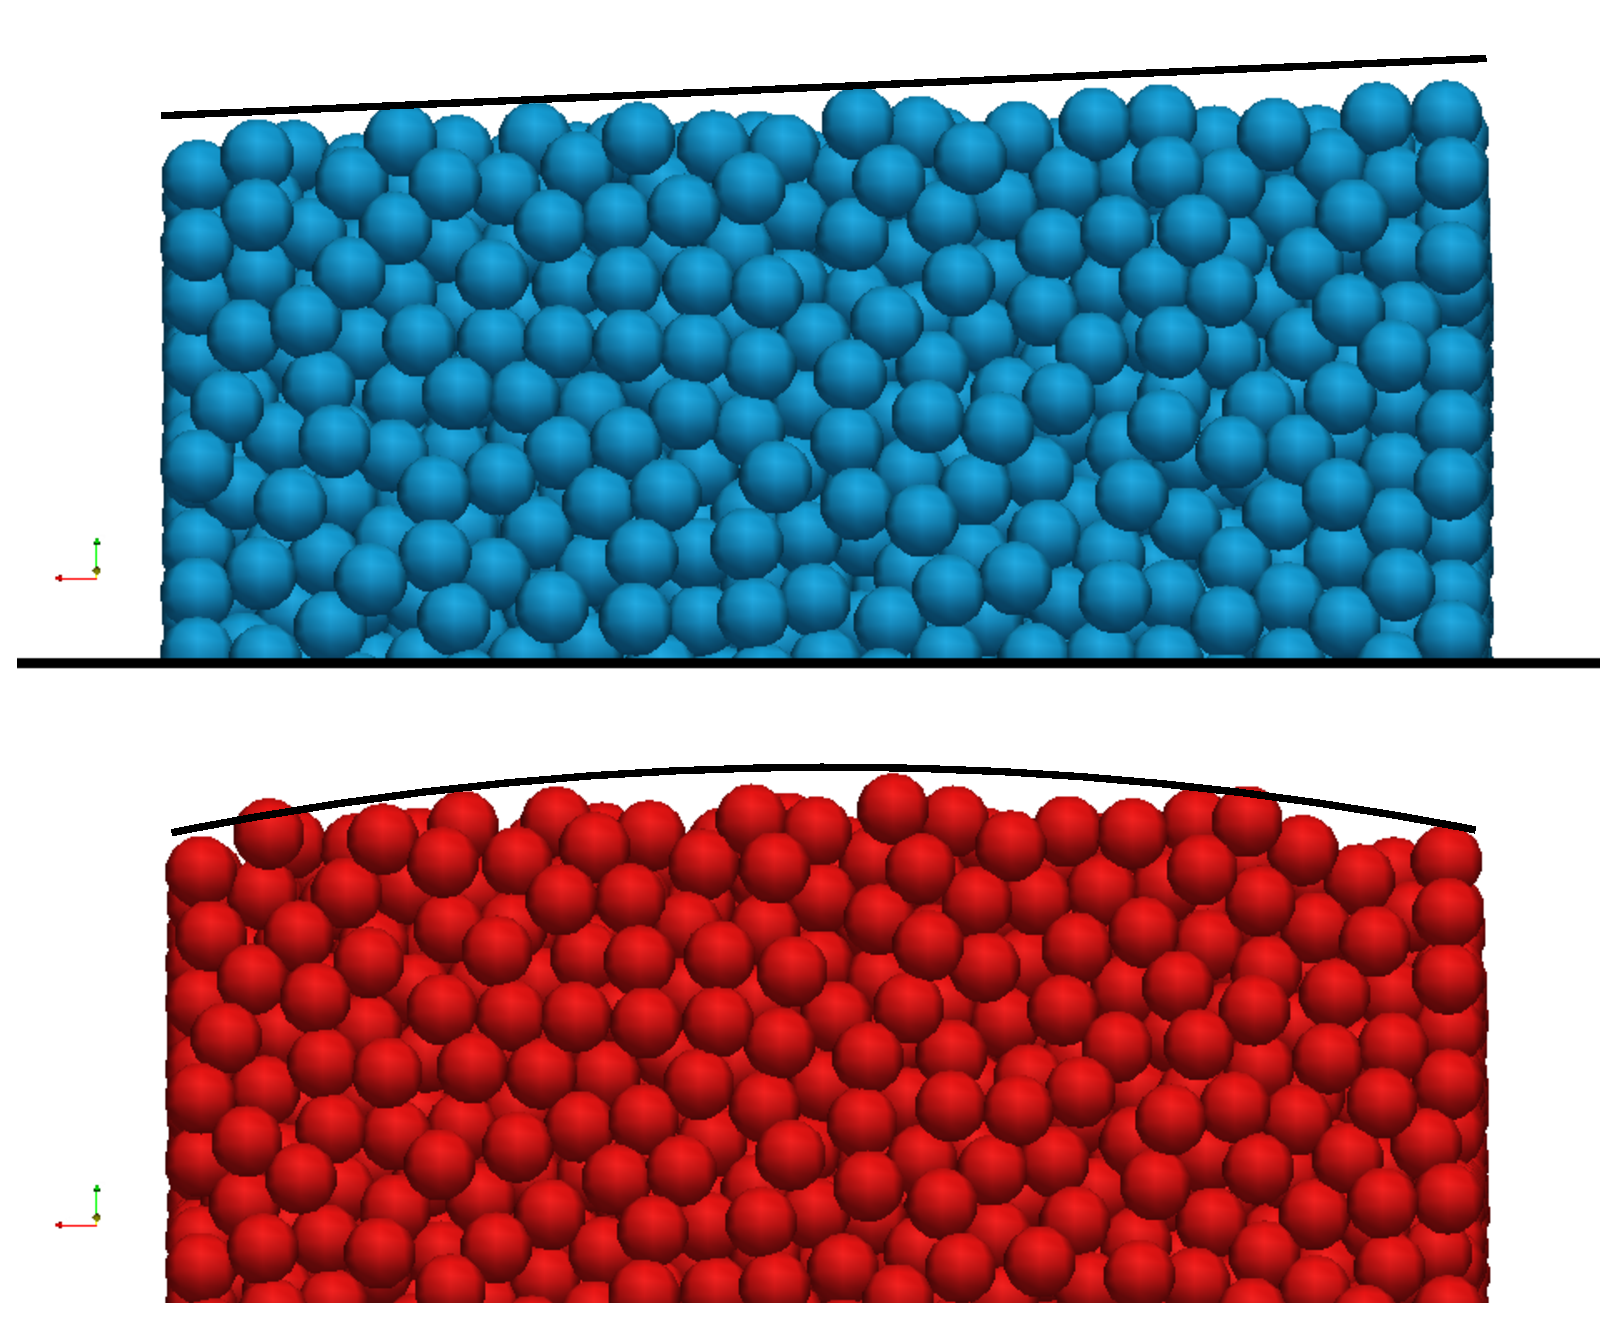
\includegraphics[width=0.4\textwidth]{chapters/figures/settlingStudy}
	\caption{Demonstrating the dynamic resettling from an example study done on location bias to pebble failure. The top image had the pebbles near the left wall biased to fail. The bottom image had a bias for the pebbles near both walls to fail. The lines are drawn as an aid to the eye.}
\label{fig:settlingStudy}
\end{figure}


The aim of this study was both to discover the impact of pebble failure on thermomechanical properties as well as determine the impact as a function of the number of failed pebbles. To satisfy the latter, we created beds with $\eta = 1\%$, $5\%$, $10\%$, and $15\%$ of pebbles failed. 

We first compare steady-state temperature profiles in the test beds against the one-dimensional theory of Eq.\ref{eq:continuum-heateqn}. To find the temperature profile in $x$, we create volumes of width $\Delta x$ that extend through the limits of the $y$- and $z$-directions. We then find the $n$ pebbles residing in the slices and take the mean value of their temperatures, $\langle T\rangle = \sum_{i}^n T_i / n$ of all pebble temperatures that have coordinates inside the slice. Below we will omit the notation $\langle T \rangle$ with the understanding that temperatures are volume-averages. Using the volume slices, we also find the average coordination number, $\langle Z \rangle = \sum_{i}^n Z_i / n$, normalized average contact force, $\langle F^* \rangle=\left[\langle F \rangle/\langle F_{bl} \rangle_\text{max}\right]^{1/3}$, and the normalized average temperature difference between pebbles in the slice, $\langle \Delta T_{ij} \rangle / (T_0 - T_s)_\text{bl}$; parameters which are discussed later.

When analytically solving Eq.~\ref{eq:thermoFirstLaw}, we introduce nondimensional temperature, $\theta_\text{1D} = (T -T_s)/(T_0-T_s)$, and spatial, $x^* = x/L$, variables and the solution becomes purely geometric; $\theta_\text{1D} = 1-x^{*2}$. We plot this theoretical solution against the temperature profiles coming from the steady-state DEM simulation in Fig.~\ref{fig:tempProfile}. We find that all our models had a nearly perfect match to a one-dimensional prediction, validating the calculation of effective thermal conductivity in this study. 

Another concern we had for pebble failure, was the phenomenon of `jamming' during resettling that would possibly leave pebbles isolated from their neighbors (apart from those they are resting upon). Such an isolated pebble would have no strong pathway for heat transfer and heat up much higher than that of its neighbors. Evidence of pebble isolation and `hot-spots' would be apparent in Fig.~\ref{fig:tempProfile} as localized deviations of data points from the quadratic profile. However, no deviations are seen in the data and we conclude that hot-spots will not be a concern in a packed bed.

\begin{figure}[t]
	\centering
	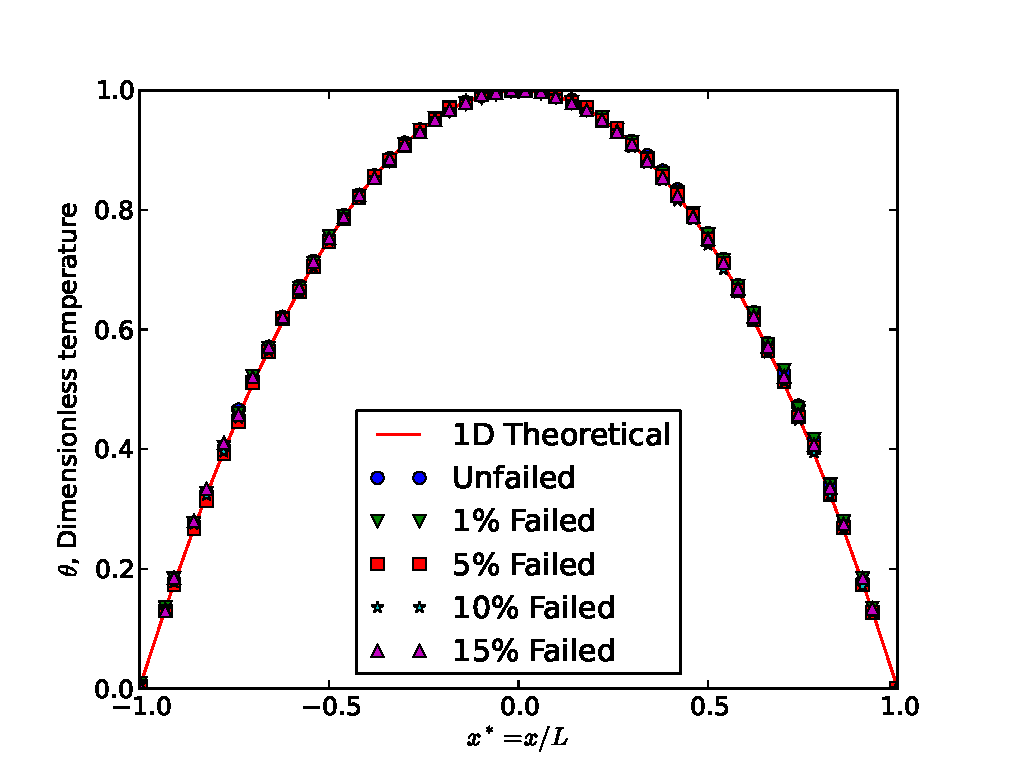
\includegraphics[width=0.5\textwidth]{chapters/figures/tempProfiles}
	\caption{The nondimensional temperature profiles for each test case follow the theoretical shape of a one-dimensional, constant $k$, continuum solution.}
\label{fig:tempProfile}
\end{figure}



\begin{figure}[t]
	\centering
	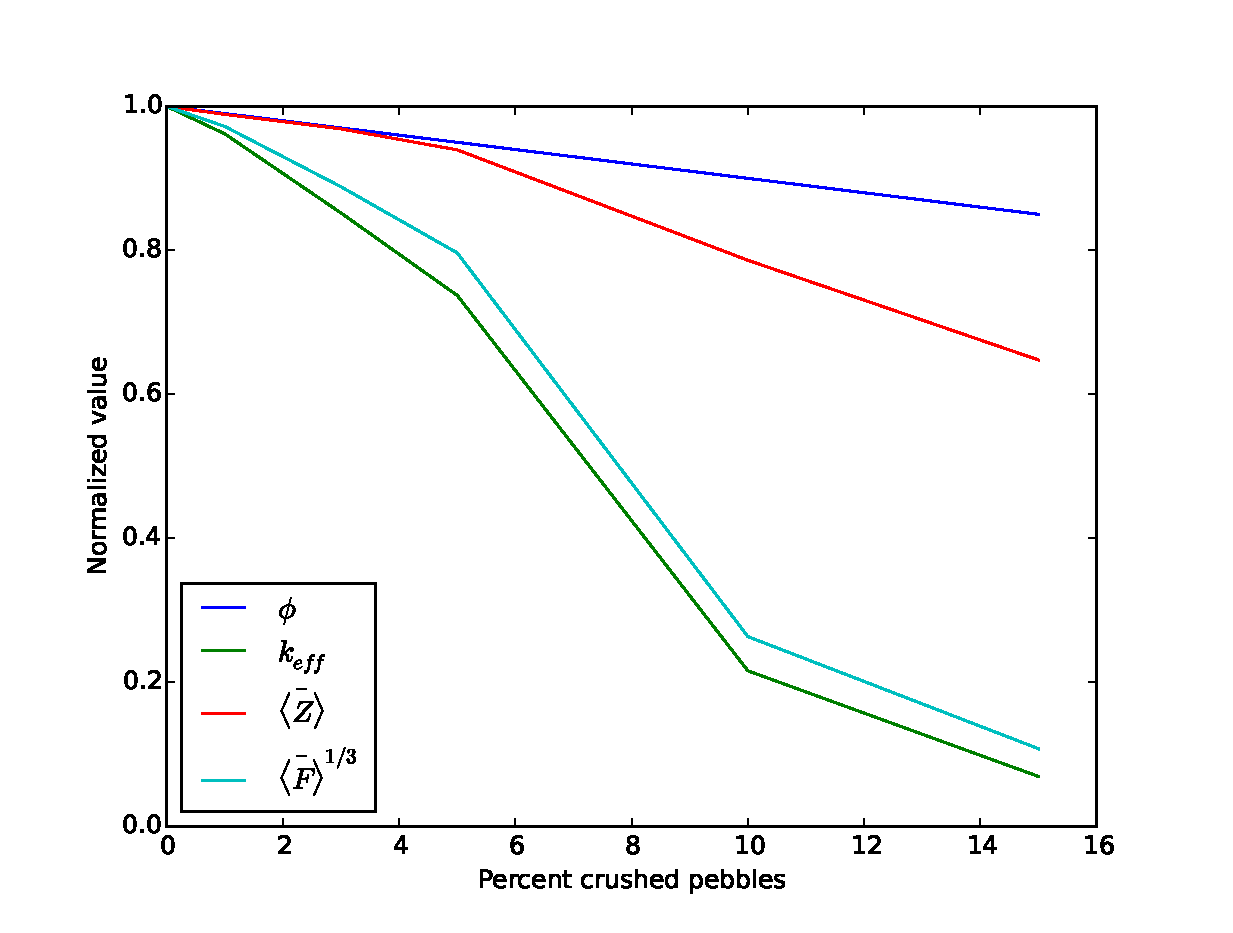
\includegraphics[width=0.5\textwidth]{chapters/figures/kEff_packingFraction}
	\caption{The normalized effective thermal conductivity (solid line) follows an exponential decay relationship with amount of failed pebbles. The normalized packing fraction (dashed line), compared to thermal conductivity, is relatively constant and is more closely fit to a linear reduction.}
\label{fig:packingFraction}
\end{figure}

\begin{figure}[t]
	\centering
	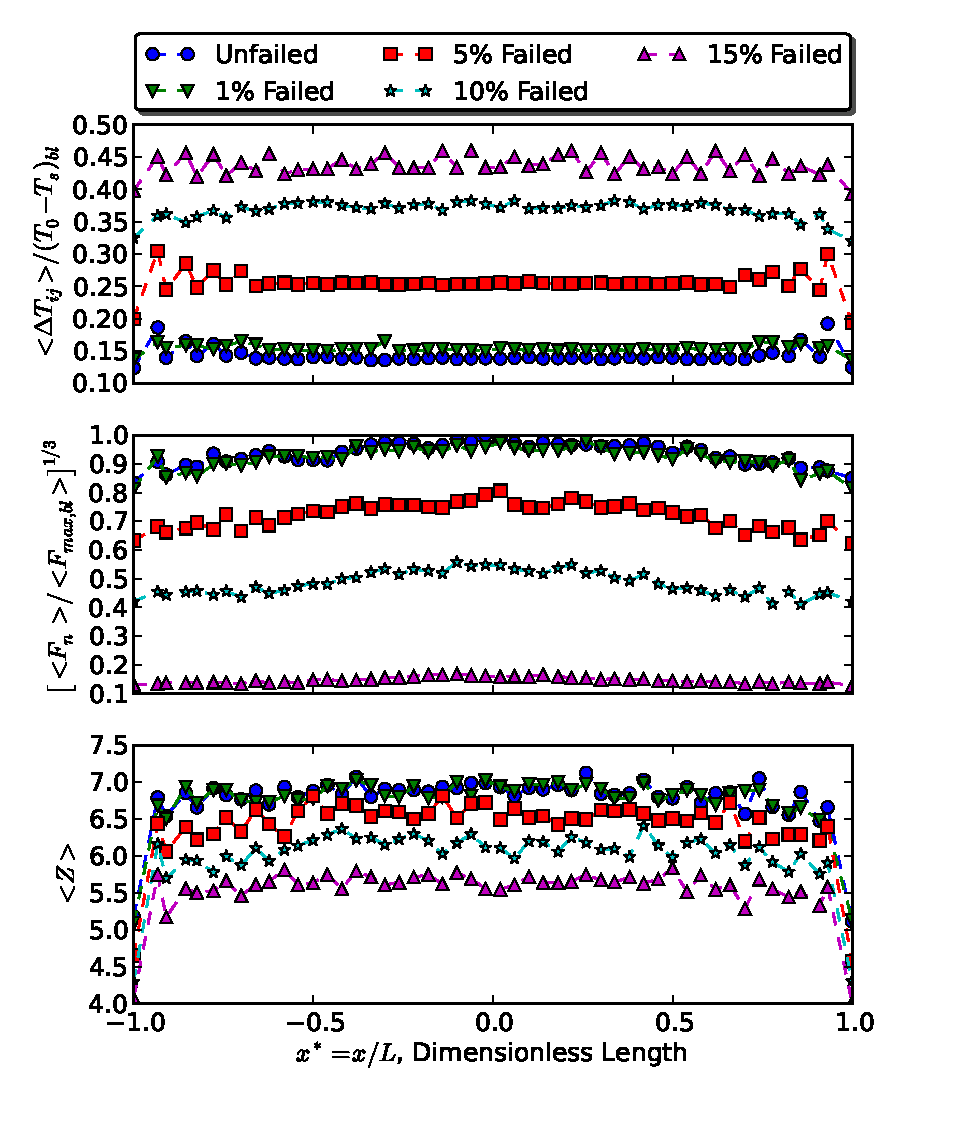
\includegraphics[width=0.5\textwidth]{chapters/figures/z_f_deltaT_subPlots}
	\caption{Average temperature differences between neighboring pebbles (top), contact forces (middle) and coordination numbers (bottom). The profiles of average coordination number and contact forces in the bed decrease in value with increasing pebble failure. Fewer and weaker contacts will reduce the possible paths of heat transfer from a pebble and this results in higher average temperatures between neighbors.}
\label{fig:coordProfiles}
\end{figure}


The effective thermal conductivity is found for all of our pebble beds, via Eq.~\ref{eq:etc}, then normalized against the conductivity of the baseline ensemble ($k_\text{eff}^* = k_\text{failed}/k_\text{bl}$). Figure~\ref{fig:packingFraction} shows the decreasing ETC with pebble failure. When $15\%$ of the pebbles are crushed in a pebble bed, the ETC has fallen all the way to only $k_\text{eff}^*=0.30$. This large reduction is especially important in light of the already poor thermal management of virgin pebble beds that, even in helium environments, have been experimentally measured at only approximately 1~W/m-K (see, { e.g.}, Refs.~\cite{Reimann:2002mi, Piazza2002}). In well-packed pebble beds, the ETC is generally related to the packing fraction. In Fig.~\ref{fig:packingFraction}, this relationship seems weak as the effective conductivity drops much more rapidly than does the packing fraction as the number of broken pebbles in the ensemble increases. To find the cause of decrease in conductivity and to make use of the information provided by DEM tools, we look to other parameters than the packing fraction.

From Eq.~\ref{eq:thermoFirstLaw}, in the steady-state, the energy input by nuclear heating must be balanced by the transport of heat out of a pebble into its neighbors. Inter-particle heat transfer is dictated by the number of neighboring contacts, temperature difference between pebbles, and the thermal conductance, $h_{ij}$ through the contact area. The thermal conductance is, itself, a function of material properties  (which are essentially constant here) and the force at the contact, going as $h_{ij} \propto F_n^{1/3}$. Thus, the net heat out is a function of the three variables as

\begin{align}
	Q_\text{net} =f( Z, F_n^{1/3}, \Delta T)
\end{align}



The variables affecting $Q_\text{net}$ are plotted in Fig.~\ref{fig:coordProfiles}. The average coordination number, shown in the bottom plot, decreases from a mid-line value of about 7.0 at the steady-state of the baseline case down to a mid-line value of 5.5 for the 15\% failed bed; a reduction of about 80\%. But this number doesn't compare with the large reduction in ETC which was $k_\text{eff}^*=0.30$. Clearly, there are fewer contacts in the pebble bed after failure but this alone does not account for the reduction in ETC.

Much more dramatic, seen in the center plot, is the reduction in average normal force seen by pebbles after many of the neighbors fail and are removed from the system. From the baseline down to the 15\% failed case, the contact forces are dramatically reduced to about $\langle F^* \rangle=0.1$.This reduction in force is joined by an increase in average neighbor temperatures which are 3 times higher for the bed with most failed pebbles when compared to the baseline. 

The results shown in Fig.~\ref{fig:coordProfiles} demonstrate that the heat transfer through a pebble bed is simultaneously a function of the coordination number and inter-particle contact forces -- which are both reduced as pebbles in the bed fail -- as well as the temperature difference between pebbles at steady state -- which increases as pebbles in the ensemble fail. Interestingly, when a pebble bed has lower overall inter-particle contact forces fewer particles would be expected to break. This would imply that pebble breakage is self-dampening; as pebbles begin to break the ensemble quickly relaxes and avoids future pebble failure. So while we induced failure up to $\eta = 15\%$, such large values may not occur in real beds. 

Another feature of Fig.~\ref{fig:coordProfiles} worth noting is the increase in averaged normal contact forces near the center of the bed relative to the walls. In the assumptions used to develop this simulation, we had noted the lack of localized force concentrations in a bed under an external mechanical load. However, in these results, owing to the nuclear heating temperature profile and thermal expansion of each pebble, there is a bias toward higher forces in the center of the bed. This result highlights the need for a model to predict failure initiation in place of the assumption of random pebble failure. 
%There are dramatic decreases near the walls for two reasons. The first being that contact of a pebble with a wall is not counted in the overall coordination number. The second is the forced ordering that pebbles experience near walls that is absent from the random packing in the bulk. Away from the walls, there is a clear decreasing trend in the coordination number as the pebble failure increases. From Eq.~\ref{eq:thermoFirstLaw}, the heat transfer from a pebble is a function of the number of neighbors with which the pebble is in contact. 



\section{Conclusions}
\label{concs}
The current study aimed at properly simulating a pebble bed with a specified fraction of the pebbles failing during operation; then determining the repercussions of the failures as they affect the macroscopic property of effective thermal conductivity. We used the assumption of homogeneous, random locations of pebble failure to induce a failure routine without requiring external loads on the bed to permit beds that could be directly compared. After heating to a steady-state, an effective thermal conductivity was calculated for the pebble bed. The results show that small amounts of pebble failure correspond to large decreases in the conductive transport of energy through the pebble bed. The increase was due primarily to a drop in the inter-particle forces which lead to a large increase in temperature differences between neighboring pebbles. We note again, however, that this value has been calculated in the absence of interstitial gas so the results apply only to the reduction in energy transferred via inter-particle conduction.


The assumption of homogeneous distribution of pebble failure was found to be inappropriate after a pebble bed reached steady state nuclear heating. The scheme assumes no localization of average forces in the bed but we found an average force profile that had a maximum at the center and minimum at the walls. The next step of modeling will eliminate the error of such an assumption as we must combine failure prediction to failure outcome modeling. 






%\input{chapters/modeling-cfdem.tex}
%\chapter{Development of lattice-Boltzmann Modeling Tools for Ceramic Solid Breeders}\label{sec:modeling-lbm}
The volume-averaged approach of the CFD-DEM coupling is an effective and efficient method for solving transiently coupled helium flow and pebble interaction. However, there are cases when a complete knowledge of the tortuous flow of the interstitial helium is desired. But because the CFD-DEM solver does not resolve the pathways on the particle scale, knowledge of precise helium flow is not possible with that technique. Therefore we have also investigated a combination of DEM and with lattice-Boltzmann solvers. 

The lattice-Boltzmann approach to fluid simulations is a growing field of numerical modeling with a rich historical development. As the LBM approach is relatively unfamiliar, we will go through some of the notable evolutions of the modeling history and the background physics leading to the governing equations to be implemented numerically. Certainly this short study cannot do justice to a proper explanation of the underlying physics. References~\cite{Chen1998a,Viggen2009,Sukop2007,Chopard2002,succi2001lattice} should be read by those curious for excellent and thorough descriptions of the physics, modeling approaches, and applications of LBM theory to fluid dynamics problems.

In the rest of this chapter we introduce the core concepts behind the lattice-Boltzmann method, their application into numerical code, and finally a discussion of the solver used in this research.

%%%%%%%%%%%%%%%%%%%%%%%%%%%%%%%%%%%%%%%%%%
\input{chapters/sections/lbm-modeling-intro.tex}
\section{Numerical Methodology}

The distribution function at a given node is explicitly updated in time in two steps: collision and streaming. In the first step, collision operator of Eq.~\ref{eq:bgk-operator} dictates the distribution function at all the nodes. In the second step, information is streamed for the timestep to neighboring nodes according to Eq.~\ref{eq:lbm-evolution}.

The collision operator for the thermal lattice is that given by Guo, et al.17 The solver has two lattices overlaid upon each other. The first is used to solve for density and velocity. The second lattice uses the velocity at each node and solves for the passive temperature scalar. 

For our model we represented the pebbles with a resolution of 10 nodes per diameter. For the system analyzed, this resulted in two lattices that have nodal sizes of 201×151×501; requiring, in a total, about 30 million nodes to be updated at each time step.

In the DEM-LBM approach, DEM is used only to determine packing structure and contact forces. When the bed is settled, a snapshot of the structure is discretized and loaded into the LBM solver which then calculates temperature and velocity fields of both solid and fluid phases. There is no cross-communication in this technique as the packing structure is effectively frozen during the LBM calculations.

\input{chapters/sections/lbm-benchmark.tex}
%%%%%%%%%%%%%%%%%%%%%%%%%%%%%%%%%%%%%%%%%%
%\input{chapters/experimenting.tex}


\appendix
\section{Sphere with heat generation}

To provide homogeneous boundary conditions, the temperature will everywhere be in reference to its difference from the fluid temperature, i.e. $\mathbb{T} = T-T_f$. 

Energy equation

\begin{equation}
    \frac{1}{r}\frac{\partial^2}{\partial r^2}(r\mathbb{T}) + \frac{g}{k} = \frac{1}{\alpha}\frac{\partial \mathbb{T}}{\partial t}
\end{equation}

Subject to 

\begin{equation}
    \frac{\partial \mathbb{T}}{\partial r}\big|_b + \frac{h}{k}\mathbb{T}|_b = 0
\end{equation}

and

\begin{equation}
    \mathbb{T}|_0 = \text{finite}
\end{equation}

with initial condition

\begin{equation}
    \mathbb{T}(r,0) = \mathbb{T}_0
\end{equation}

Transform with 

\begin{equation}
    U(r,t) = r\mathbb{T}(r,t)
\end{equation}

Energy equation becomes

\begin{equation}
    \frac{\partial^2 U}{\partial r^2} + \frac{gr}{k} = \frac{1}{\alpha}\frac{\partial U}{\partial t}
\end{equation}

Subject to

\begin{equation}
    \frac{\partial U}{\partial r}\big|_b + \left(\frac{h}{k} - \frac{1}{b}\right)U|_b = \frac{hb}{k}T_f
\end{equation}

and

\begin{equation}
    U|_0 = 0
\end{equation}

with initial condition

\begin{equation}
    U(r,0) = T_0r
\end{equation}

Break up the problem into simpler problems

\begin{enumerate}
\item A set of steady-state problems defined by $U_{ss}(r)$
\item A homogeneous time-dependent problem defined by $U_h(r,t)$
\end{enumerate}

The solution of $U_{ss}$ is found from the solution of

\begin{equation}
    \frac{\partial^2 U_{ss}}{\partial r^2} + \frac{gr}{k} = 0
\end{equation}

subject to the boundary conditions of
\begin{align}\label{eq:ss-bcs}
    U_{ss}\big|_0 &= 0\\
    \frac{\partial U_{ss}}{\partial r}\big|_b + \left(\frac{h}{k} - \frac{1}{b}\right)U_{ss}\big|_b &= 0
\end{align}

We separate and integrate, 

\begin{align}
    \frac{\partial U_{ss}}{\partial r} & = -\frac{g}{2k} r^2 + C_1\\
    U_{ss} & = -\frac{g}{6k} r^3 + C_1r + C_2
\end{align}

The first boundary condition of Eq.~\ref{eq:ss-bcs} directly provides $C_2 = 0$. The second boundary condition is solved to give

\begin{equation}
    C_1 = \frac{gb^2}{6k}\left(1 + \frac{2}{Bi}\right)
\end{equation}

valid for $Bi > 0$. Thus,

\begin{equation}
    U_{ss} = \frac{gb^2}{6k}\left(1 + \frac{2}{Bi}-\frac{r^2}{b^2}\right)r
\end{equation}

We can now transform back to the temperature version of the equation with the simple reduction in power of $r$ on U, (U = r$\mathbb{T}$),

\begin{equation}
    \mathbb{T}_{ss} = \frac{gb^2}{6k}\left(1 + \frac{2}{Bi}-\frac{r^2}{b^2}\right) 
\end{equation}

Now we non-dimensionalize with 

\begin{equation}\label{eq:dimensionless-temp-definition}
    \theta = \frac{\mathbb{T}}{gb^2/k}
\end{equation}

and

\begin{equation}
    r^* = \frac{r}{b}
\end{equation}


\begin{equation}
    \theta_{ss} = \frac{1}{6} \left( 1 + \frac{2}{Bi} - r^{*2} \right)
\end{equation}

The next step is to find the homogeneous solution of 

\begin{equation}
    \frac{\partial^2 U_h}{\partial r^2} = \frac{1}{\alpha}\frac{\partial U_h}{\partial t}
\end{equation}

Subject to 

\begin{align}
    U_{h}\big|_0 &= 0\\
    \frac{\partial U_{h}}{\partial r}\big|_b + \left(\frac{h}{k} - \frac{1}{b}\right)U_{h}\big|_b &= 0
\end{align}

and the initial condition of

\begin{align}
    U_{h,0} &= \mathbb{T}_0r - U_{ss}\\
    & = \left[\frac{\mathbb{T}_0}{gb^2/k} - \frac{1}{6}\left(1 + \frac{2}{Bi} - \frac{r^2}{b^2}\right)\right]r
\end{align}

We will again transform the spatial variable into a dimensionless form, $r^* = r/b$. The equation to solve is then,

\begin{equation}
    \frac{\partial^2 U_h}{\partial r^{*2}} = \frac{b^2}{\alpha}\frac{\partial U_h}{\partial t}
\end{equation}

with boundary conditions of

\begin{align}
    U_{h}\big|_0 &= 0\\
    \frac{\partial U_{h}}{\partial r^*}\big|_1 + (Bi - 1)U_{h}\big|_1 &= 0
\end{align}

and an initial condition of

\begin{align}
    U_h(t=0) &= T_0r^*b - \sum_{j=0}^N U_{0j}\\
    & = \left[\frac{\mathbb{T}_0}{gb^2/k} - \frac{1}{6}\left(1 + \frac{2}{Bi} - r^*\right)\right]r^*b
\end{align}


The solution is assumed of the form

\begin{equation}
    U_h = R(r^*) \Gamma(t)
\end{equation}

The solution for $\Gamma$ is given as

\begin{equation}
    \Gamma = \exp(-\zeta^2t/\tau)
\end{equation}

where $\tau = b^2/\alpha$. The space-variable function $R(\zeta,r^*)$ satisfies the following eigenvalue problem:

\begin{equation}\label{eq:eigen-function}
    \frac{\mathrm{d}^2R}{\mathrm{d}r^{*2}} + \zeta^2 R = 0
\end{equation}

subject to 

\begin{equation}
    R = 0
\end{equation}

at $r^* = 0$, and

\begin{equation}
    \frac{\mathrm{d}R}{\mathrm{d}r^*} + (Bi - 1)R = 0
\end{equation}

at $r^* = 1$. This eigenvalue problem is a special case of the Sturm-Liouville problem. The solution for $U_h$ can be constructed from known eigenvalue solutions,

\begin{equation}\label{eq:eigen-general-solution}
    U(r,t) = \sum_{n=1}^\infty c_n R(\zeta_n,r^*)\exp(-\zeta^2 t/\tau)
\end{equation}

Application of the initial condition gives

\begin{equation}\label{eq:eigen-initial-condition}
    F(r) = \sum_{n=1}^\infty c_n R(\zeta_n,r^*)
\end{equation}

where $F(r^*)$ is the initial condition we defined above, 

\begin{equation}
    F(r^*) =\left[\frac{\mathbb{T}_0}{gb^2/k} - \frac{1}{6}\left(1 + \frac{2}{Bi} - r^*\right)\right]\frac{gb^2}{k}r^*b 
\end{equation}

The coefficients of $c_n$ can be determined by applying the operator $\int_0^1 R(\zeta_n,r^*)\,\mathrm{d}r^*$ and utilizing the orthogonality property of eigenfunctions. The coefficients are found as

\begin{equation}\label{eq:eigenfunction-coefficients}
    c_n = \frac{1}{N(\zeta_n)}\int_0^1 R(\zeta_n,r^{*'})F(r^{*'})\,\mathrm{d}r^{*'}
\end{equation}

The norm, $N$ is defined as

\begin{equation}
    N(\zeta_n) = \int_0^1 \left[R(\zeta_n,r^*)\right]^2\,\mathrm{d}r^*
\end{equation}

With the coefficients defined in Eq.~\ref{eq:eigenfunction-coefficients}, they can be substituted back into Eq.~\ref{eq:eigen-general-solution},

\begin{equation}
    U(r^*,t) = \sum_{n=1}^\infty \exp(-\zeta^2 t/\tau) \frac{R(\zeta_n,r^*)}{N(\zeta_n)}\int_0^1 R(\zeta_n,r^{*'})F(r^{*'})\,\mathrm{d}r^{*'}
\end{equation}

% Eq.~\ref{eq:eigenfunction-coefficients} is also inserted back into Eq.~\ref{eq:eigen-initial-condition},

% \begin{equation}
%     (T_0-T_f)r - \frac{g}{6k} r^3 - \frac{gb^2}{6k}\left(1 + \frac{2}{Bi}\right)r = \sum_{n=1}^\infty \frac{R(\zeta_n,r)}{N(\zeta_n)}\int_0^b R(\zeta_n,r')F(r')\,\mathrm{d}r'
% \end{equation}

The eigenfunctions for Eq.~\ref{eq:eigen-function} are

\begin{equation}
    R(\zeta_n,r^*) = \sin(\zeta_n r^*)
\end{equation}

where the eigenvalues are the root of

\begin{equation}
    \zeta_n\cot(\zeta_n) = -H
\end{equation}

and the normalization integral is given as

\begin{equation}
    \frac{1}{N(\zeta_n)} = 2\frac{\zeta_n^2 + H^2}{\zeta_n^2+H^2 + H}
\end{equation}

where $H = (Bi-1)$

In order to explicitly express the solution, we will first evaluate the integral

\begin{align}
    Z(\zeta_n)\frac{gb^2}{k}b & = \int_0^1 R(\zeta_n,r^{*'})F(r^{*'})\,\mathrm{d}r^{*'} \\
    & = \int_0^1\sin(\zeta_nr^{*'}) \left[\frac{\mathbb{T}_0}{gb^2/k} - \frac{1}{6}\left(1 + \frac{2}{Bi} - r^*\right)\right]r^*b \,\mathrm{d}r^{*'}\\
    & =\left\{ \left[\frac{\mathbb{T}_0}{gb^2/k}  - \frac{1}{6}\left(1 + \frac{2}{Bi}\right)\right]\int_0^1\sin(\zeta_nr^{*'})r^{*'} \,\mathrm{d}r^{*'} + \frac{1}{6}\int_0^1 \sin(\zeta_nr^{*'})r^{*'3} \,\mathrm{d}r^{*'}\right\}\frac{gb^2}{k}b
\end{align}

The two unique integrals are evaluated as

\begin{align}
    C_n &= \int_0^1\sin(\zeta_nr^{*'})r^{*'} \,\mathrm{d}r^{*'}  = \frac{\sin\zeta_n-\zeta_n\cos\zeta_n}{\zeta_n^2}\\
    K_n &= \int_0^1\sin(\zeta_nr^{*'})r^{*'3} \,\mathrm{d}r^{*'}  = \frac{3(\zeta_n^2-2)\sin\zeta_n - \zeta_n(\zeta_n^2-6)\cos\zeta_n}{\zeta_n^4}
\end{align}

Thus
\begin{equation}
    Z(\zeta_n) = \left[\frac{\mathbb{T}_0}{gb^2/k} - \frac{1}{6}\left(1 + \frac{2}{Bi}\right)\right]C_n + \frac{1}{6}K_n
\end{equation}

or in terms of our dimensionless temperature,
\begin{equation}
    Z(\zeta_n) = \left[\theta_0 - \frac{1}{6}\left(1 + \frac{2}{Bi}\right)\right]C_n + \frac{1}{6}K_n
\end{equation}

The solution in terms of the transformed variable, $U(r^*,T)$ is now written as

\begin{equation}
    U(r^*,t) = \sum_{n=1}^\infty \exp(-\zeta^2 t/\tau) \sin(\zeta_n r^*)\frac{Z(\zeta_n)\frac{gb^2}{k}b}{N(\zeta_n)}
\end{equation}

Now we can write the solution for $\mathbb{T}(r^*,t)$ direclty from $U(r^*,t)$,

\begin{equation}
    \mathbb{T}(r^*,t) = \sum_{n=1}^\infty \exp(-\zeta^2 t/\tau) \frac{\sin(\zeta_n r^*)}{r^*}\frac{Z(\zeta_n)\frac{gb^2}{k}}{N(\zeta_n)}
\end{equation}

With one last step, we introduce the dimensionless temperature defined from Eq.~\ref{eq:dimensionless-temp-definition}

\begin{equation}
    \theta(r^*,t)_{t.g.} = \sum_{n=1}^\infty \exp(-\zeta^2 t/\tau) \frac{\sin(\zeta_n r^*)}{r^*}\frac{Z(\zeta_n)}{N(\zeta_n)}
\end{equation}



For comparison, we will non-dimensionalize the heat transfer as:

\begin{equation}
    Q^*=\frac{Q}{Q_{\infty}}
\end{equation}

where $Q_{\infty}$ is the maximum possible amount of energy transfer between the solid and fluid.  This value is equal for both lumped capacitance and the exact solution and is:

\begin{equation}
    Q_{\infty}=-\rho_rC_rV(T_f - T_i)
\end{equation}

Introducing this non-dimensional heat transfer term and the energy balance is expressed as: 

\begin{align}
    Q^*_{t.g.}&=\int\frac{-\rho_rC_r\big(T(r,t)-T_0\big)dV}{-\rho_rC_rV(T_{\infty}-T_0)}\\
    Q^*_{t.g.}&=\frac{1}{V}\int 1 - \theta_{t.g.} \,\mathrm{d}V
\end{align}


For a circle in spherical coordinates:

\begin{equation}
    \mathrm{d}V=r^2\sin(\phi)\mathrm{d}r\mathrm{d}\phi \mathrm{d}\theta
\end{equation}

In non-dimensional terms and assuming only a radial dependence, this becomes:

\begin{equation}
    \mathrm{d}V=4\pi R^3 r^{*2}\mathrm{d}r^*
\end{equation}

The exact equation for dimensionless heat transfer for a sphere is then:

\begin{equation}
    Q^*_{t.g.}=\frac{4\pi R^3}{V}\int_0^1  \left[ 1 -\sum_{n=1}^\infty \exp(-\zeta^2 t/\tau) \frac{\sin(\zeta_n r^*)}{r^*}\frac{Z(\zeta_n)}{N(\zeta_n)} \right] r^{*2}\,\mathrm{d}r^*
\end{equation}

This reduces to:

\begin{equation}
    Q^*_{t.g.}=1 - 3\sum_{n=1}^\infty \exp(-\zeta^2 t/\tau) \frac{Z(\zeta_n)}{N(\zeta_n)} \int_0^1 r^* \sin(\zeta_n r^*)\,\mathrm{d}r^* 
\end{equation}

And we recognize the integral as one which we solved previously,

\begin{equation}
\label{eq:qexact}
    Q^*_{t.g.}=1 - 3\sum_{n=1}^\infty \exp(-\zeta^2 t/\tau) \frac{Z(\zeta_n)}{N(\zeta_n)} C_n(\zeta_n)
\end{equation}

And we are left with a formula for the total heat removed from the sphere as only a function of the eigenvalues and time.


%\input{Appendix6.tex}


\bibliographystyle{ieee}
\bibliography{library}
\end{document}
